\documentclass[1p]{elsarticle_modified}
%\bibliographystyle{elsarticle-num}

%\usepackage[colorlinks]{hyperref}
%\usepackage{abbrmath_seonhwa} %\Abb, \Ascr, \Acal ,\Abf, \Afrak
\usepackage{amsfonts}
\usepackage{amssymb}
\usepackage{amsmath}
\usepackage{amsthm}
\usepackage{scalefnt}
\usepackage{amsbsy}
\usepackage{kotex}
\usepackage{caption}
\usepackage{subfig}
\usepackage{color}
\usepackage{graphicx}
\usepackage{xcolor} %% white, black, red, green, blue, cyan, magenta, yellow
\usepackage{float}
\usepackage{setspace}
\usepackage{hyperref}

\usepackage{tikz}
\usetikzlibrary{arrows}

\usepackage{multirow}
\usepackage{array} % fixed length table
\usepackage{hhline}

%%%%%%%%%%%%%%%%%%%%%
\makeatletter
\renewcommand*\env@matrix[1][\arraystretch]{%
	\edef\arraystretch{#1}%
	\hskip -\arraycolsep
	\let\@ifnextchar\new@ifnextchar
	\array{*\c@MaxMatrixCols c}}
\makeatother %https://tex.stackexchange.com/questions/14071/how-can-i-increase-the-line-spacing-in-a-matrix
%%%%%%%%%%%%%%%

\usepackage[normalem]{ulem}

\newcommand{\msout}[1]{\ifmmode\text{\sout{\ensuremath{#1}}}\else\sout{#1}\fi}
%SOURCE: \msout is \stkout macro in https://tex.stackexchange.com/questions/20609/strikeout-in-math-mode

\newcommand{\cancel}[1]{
	\ifmmode
	{\color{red}\msout{#1}}
	\else
	{\color{red}\sout{#1}}
	\fi
}

\newcommand{\add}[1]{
	{\color{blue}\uwave{#1}}
}

\newcommand{\replace}[2]{
	\ifmmode
	{\color{red}\msout{#1}}{\color{blue}\uwave{#2}}
	\else
	{\color{red}\sout{#1}}{\color{blue}\uwave{#2}}
	\fi
}

\newcommand{\Sol}{\mathcal{S}} %segment
\newcommand{\D}{D} %diagram
\newcommand{\A}{\mathcal{A}} %arc


%%%%%%%%%%%%%%%%%%%%%%%%%%%%%5 test

\def\sl{\operatorname{\textup{SL}}(2,\Cbb)}
\def\psl{\operatorname{\textup{PSL}}(2,\Cbb)}
\def\quan{\mkern 1mu \triangleright \mkern 1mu}

\theoremstyle{definition}
\newtheorem{thm}{Theorem}[section]
\newtheorem{prop}[thm]{Proposition}
\newtheorem{lem}[thm]{Lemma}
\newtheorem{ques}[thm]{Question}
\newtheorem{cor}[thm]{Corollary}
\newtheorem{defn}[thm]{Definition}
\newtheorem{exam}[thm]{Example}
\newtheorem{rmk}[thm]{Remark}
\newtheorem{alg}[thm]{Algorithm}

\newcommand{\I}{\sqrt{-1}}
\begin{document}

%\begin{frontmatter}
%
%\title{Boundary parabolic representations of knots up to 8 crossings}
%
%%% Group authors per affiliation:
%\author{Yunhi Cho} 
%\address{Department of Mathematics, University of Seoul, Seoul, Korea}
%\ead{yhcho@uos.ac.kr}
%
%
%\author{Seonhwa Kim} %\fnref{s_kim}}
%\address{Center for Geometry and Physics, Institute for Basic Science, Pohang, 37673, Korea}
%\ead{ryeona17@ibs.re.kr}
%
%\author{Hyuk Kim}
%\address{Department of Mathematical Sciences, Seoul National University, Seoul 08826, Korea}
%\ead{hyukkim@snu.ac.kr}
%
%\author{Seokbeom Yoon}
%\address{Department of Mathematical Sciences, Seoul National University, Seoul, 08826,  Korea}
%\ead{sbyoon15@snu.ac.kr}
%
%\begin{abstract}
%We find all boundary parabolic representation of knots up to 8 crossings.
%
%\end{abstract}
%\begin{keyword}
%    \MSC[2010] 57M25 
%\end{keyword}
%
%\end{frontmatter}

%\linenumbers
%\tableofcontents
%
\newcommand\colored[1]{\textcolor{white}{\rule[-0.35ex]{0.8em}{1.4ex}}\kern-0.8em\color{red} #1}%
%\newcommand\colored[1]{\textcolor{white}{ #1}\kern-2.17ex	\textcolor{white}{ #1}\kern-1.81ex	\textcolor{white}{ #1}\kern-2.15ex\color{red}#1	}

{\Large $\underline{12a_{1190}~(K12a_{1190})}$}

\setlength{\tabcolsep}{10pt}
\renewcommand{\arraystretch}{1.6}
\vspace{1cm}\begin{tabular}{m{100pt}>{\centering\arraybackslash}m{274pt}}
\multirow{5}{120pt}{
	\centering
	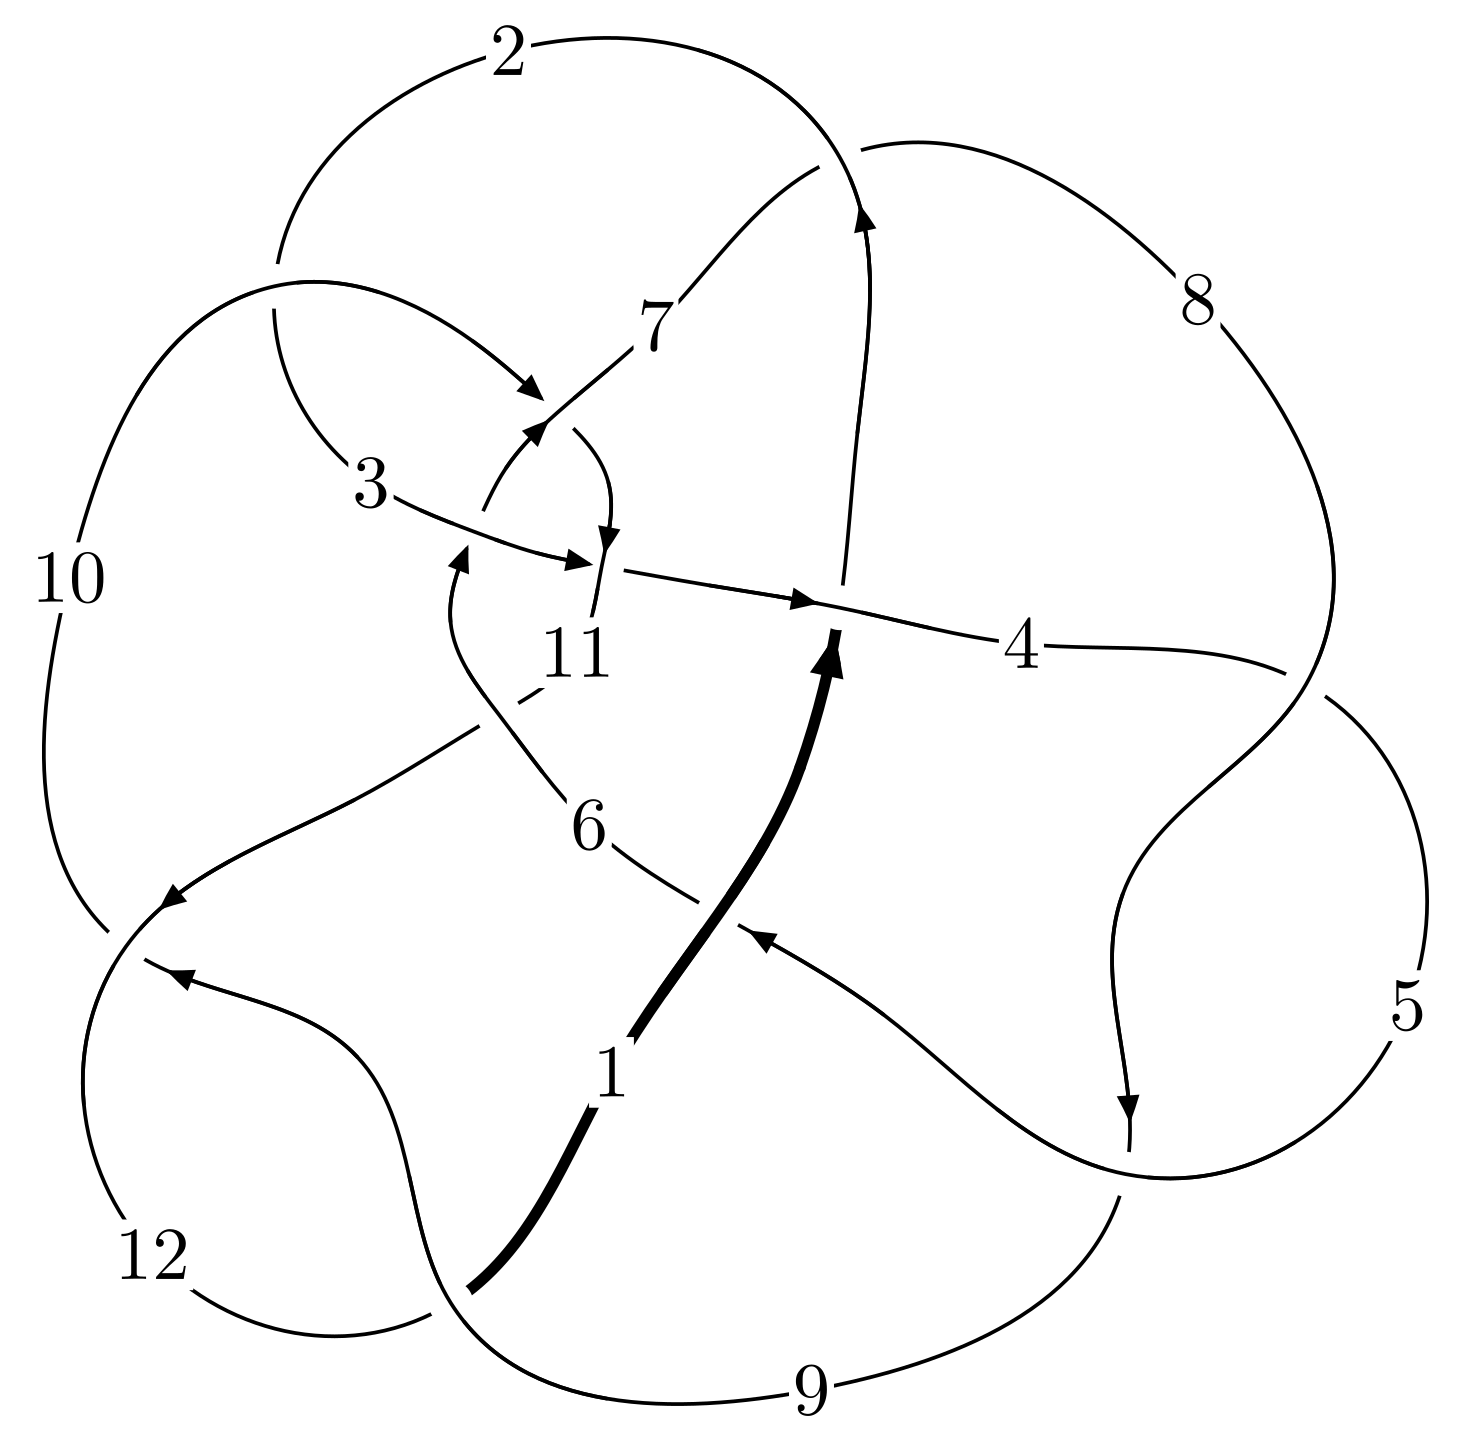
\includegraphics[width=112pt]{../../../GIT/diagram.site/Diagrams/png/1991_12a_1190.png}\\
\ \ \ A knot diagram\footnotemark}&
\allowdisplaybreaks
\textbf{Linearized knot diagam} \\
\cline{2-2}
 &
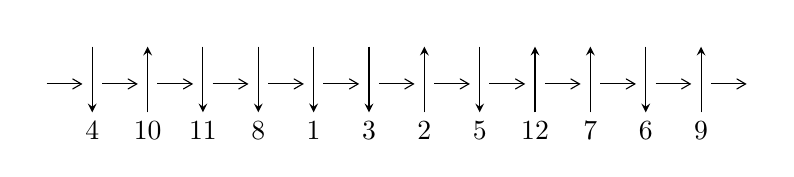
\begin{tikzpicture}[x=20pt, y=17pt]
	% nodes
	\node (C0) at (0, 0) {};
	\node (C1) at (1, 0) {};
	\node (C1U) at (1, +1) {};
	\node (C1D) at (1, -1) {4};

	\node (C2) at (2, 0) {};
	\node (C2U) at (2, +1) {};
	\node (C2D) at (2, -1) {10};

	\node (C3) at (3, 0) {};
	\node (C3U) at (3, +1) {};
	\node (C3D) at (3, -1) {11};

	\node (C4) at (4, 0) {};
	\node (C4U) at (4, +1) {};
	\node (C4D) at (4, -1) {8};

	\node (C5) at (5, 0) {};
	\node (C5U) at (5, +1) {};
	\node (C5D) at (5, -1) {1};

	\node (C6) at (6, 0) {};
	\node (C6U) at (6, +1) {};
	\node (C6D) at (6, -1) {3};

	\node (C7) at (7, 0) {};
	\node (C7U) at (7, +1) {};
	\node (C7D) at (7, -1) {2};

	\node (C8) at (8, 0) {};
	\node (C8U) at (8, +1) {};
	\node (C8D) at (8, -1) {5};

	\node (C9) at (9, 0) {};
	\node (C9U) at (9, +1) {};
	\node (C9D) at (9, -1) {12};

	\node (C10) at (10, 0) {};
	\node (C10U) at (10, +1) {};
	\node (C10D) at (10, -1) {7};

	\node (C11) at (11, 0) {};
	\node (C11U) at (11, +1) {};
	\node (C11D) at (11, -1) {6};

	\node (C12) at (12, 0) {};
	\node (C12U) at (12, +1) {};
	\node (C12D) at (12, -1) {9};
	\node (C13) at (13, 0) {};

	% arrows
	\draw[->,>={angle 60}]
	(C0) edge (C1) (C1) edge (C2) (C2) edge (C3) (C3) edge (C4) (C4) edge (C5) (C5) edge (C6) (C6) edge (C7) (C7) edge (C8) (C8) edge (C9) (C9) edge (C10) (C10) edge (C11) (C11) edge (C12) (C12) edge (C13) ;	\draw[->,>=stealth]
	(C1U) edge (C1D) (C2D) edge (C2U) (C3U) edge (C3D) (C4U) edge (C4D) (C5U) edge (C5D) (C6U) edge (C6D) (C7D) edge (C7U) (C8U) edge (C8D) (C9D) edge (C9U) (C10D) edge (C10U) (C11U) edge (C11D) (C12D) edge (C12U) ;
	\end{tikzpicture} \\
\hhline{~~} \\& 
\textbf{Solving Sequence} \\ \cline{2-2} 
 &
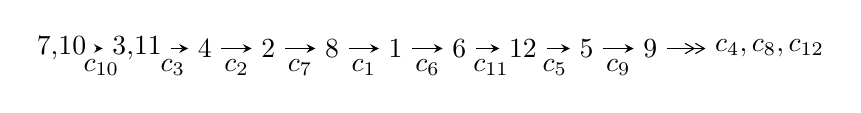
\begin{tikzpicture}[x=23pt, y=7pt]
	% node
	\node (A0) at (-1/8, 0) {7,10};
	\node (A1) at (17/16, 0) {3,11};
	\node (A2) at (17/8, 0) {4};
	\node (A3) at (25/8, 0) {2};
	\node (A4) at (33/8, 0) {8};
	\node (A5) at (41/8, 0) {1};
	\node (A6) at (49/8, 0) {6};
	\node (A7) at (57/8, 0) {12};
	\node (A8) at (65/8, 0) {5};
	\node (A9) at (73/8, 0) {9};
	\node (C1) at (1/2, -1) {$c_{10}$};
	\node (C2) at (13/8, -1) {$c_{3}$};
	\node (C3) at (21/8, -1) {$c_{2}$};
	\node (C4) at (29/8, -1) {$c_{7}$};
	\node (C5) at (37/8, -1) {$c_{1}$};
	\node (C6) at (45/8, -1) {$c_{6}$};
	\node (C7) at (53/8, -1) {$c_{11}$};
	\node (C8) at (61/8, -1) {$c_{5}$};
	\node (C9) at (69/8, -1) {$c_{9}$};
	\node (A10) at (11, 0) {$c_{4},c_{8},c_{12}$};

	% edge
	\draw[->,>=stealth]	
	(A0) edge (A1) (A1) edge (A2) (A2) edge (A3) (A3) edge (A4) (A4) edge (A5) (A5) edge (A6) (A6) edge (A7) (A7) edge (A8) (A8) edge (A9) ;
	\draw[->>,>={angle 60}]	
	(A9) edge (A10);
\end{tikzpicture} \\ 

\end{tabular} \\

\footnotetext{
The image of knot diagram is generated by the software ``\textbf{Draw programme}" developed by Andrew Bartholomew(\url{http://www.layer8.co.uk/maths/draw/index.htm\#Running-draw}), where we modified some parts for our purpose(\url{https://github.com/CATsTAILs/LinksPainter}).
}\phantom \\ \newline 
\centering \textbf{Ideals for irreducible components\footnotemark of $X_{\text{par}}$} 
 
\begin{align*}
I^u_{1}&=\langle 
-1.49146\times10^{1687} u^{177}-5.62173\times10^{1687} u^{176}+\cdots+1.88308\times10^{1688} b+1.61526\times10^{1688},\\
\phantom{I^u_{1}}&\phantom{= \langle  }-1.19578\times10^{1688} u^{177}-6.33495\times10^{1688} u^{176}+\cdots+1.12985\times10^{1689} a+1.06401\times10^{1690},\\
\phantom{I^u_{1}}&\phantom{= \langle  }u^{178}+4 u^{177}+\cdots-21 u-2\rangle \\
I^u_{2}&=\langle 
8.62429\times10^{50} u^{36}-4.71449\times10^{51} u^{35}+\cdots+1.82706\times10^{52} b+2.16797\times10^{52},\\
\phantom{I^u_{2}}&\phantom{= \langle  }1.72012\times10^{53} u^{36}+7.10407\times10^{53} u^{35}+\cdots+5.48117\times10^{52} a-3.27600\times10^{53},\;u^{37}+4 u^{36}+\cdots-6 u^2-1\rangle \\
I^u_{3}&=\langle 
b+1,\;4 a+u+1,\;u^2- u+2\rangle \\
\\
\end{align*}
\raggedright * 3 irreducible components of $\dim_{\mathbb{C}}=0$, with total 217 representations.\\
\footnotetext{All coefficients of polynomials are rational numbers. But the coefficients are sometimes approximated in decimal forms when there is not enough margin.}
\newpage
\renewcommand{\arraystretch}{1}
\centering \section*{I. $I^u_{1}= \langle -1.49\times10^{1687} u^{177}-5.62\times10^{1687} u^{176}+\cdots+1.88\times10^{1688} b+1.62\times10^{1688},\;-1.20\times10^{1688} u^{177}-6.33\times10^{1688} u^{176}+\cdots+1.13\times10^{1689} a+1.06\times10^{1690},\;u^{178}+4 u^{177}+\cdots-21 u-2 \rangle$}
\flushleft \textbf{(i) Arc colorings}\\
\begin{tabular}{m{7pt} m{180pt} m{7pt} m{180pt} }
\flushright $a_{7}=$&$\begin{pmatrix}0\\u\end{pmatrix}$ \\
\flushright $a_{10}=$&$\begin{pmatrix}1\\0\end{pmatrix}$ \\
\flushright $a_{3}=$&$\begin{pmatrix}0.105836 u^{177}+0.560692 u^{176}+\cdots-11.6907 u-9.41733\\0.0792032 u^{177}+0.298540 u^{176}+\cdots-2.76824 u-0.857776\end{pmatrix}$ \\
\flushright $a_{11}=$&$\begin{pmatrix}1\\- u^2\end{pmatrix}$ \\
\flushright $a_{4}=$&$\begin{pmatrix}0.0122961 u^{177}+0.233061 u^{176}+\cdots-12.0185 u-8.83425\\0.0760799 u^{177}+0.295925 u^{176}+\cdots-3.55824 u-0.950832\end{pmatrix}$ \\
\flushright $a_{2}=$&$\begin{pmatrix}0.0266326 u^{177}+0.262152 u^{176}+\cdots-8.92250 u-8.55956\\0.0792032 u^{177}+0.298540 u^{176}+\cdots-2.76824 u-0.857776\end{pmatrix}$ \\
\flushright $a_{8}=$&$\begin{pmatrix}-0.618581 u^{177}-2.17190 u^{176}+\cdots+52.4006 u-0.0257066\\0.176218 u^{177}+0.737382 u^{176}+\cdots-15.0884 u-2.55881\end{pmatrix}$ \\
\flushright $a_{1}=$&$\begin{pmatrix}-0.253660 u^{177}-1.02149 u^{176}+\cdots+36.8667 u+0.0634775\\0.0754801 u^{177}+0.277632 u^{176}+\cdots-5.33836 u-0.844349\end{pmatrix}$ \\
\flushright $a_{6}=$&$\begin{pmatrix}-0.255051 u^{177}-0.664552 u^{176}+\cdots+20.5289 u-5.22424\\0.187312 u^{177}+0.769967 u^{176}+\cdots-14.7832 u-2.63972\end{pmatrix}$ \\
\flushright $a_{12}=$&$\begin{pmatrix}-1.88497 u^{177}-7.51745 u^{176}+\cdots+117.974 u+36.5488\\-0.0838975 u^{177}-0.335890 u^{176}+\cdots+3.14355 u+2.04874\end{pmatrix}$ \\
\flushright $a_{5}=$&$\begin{pmatrix}-1.49126 u^{177}-5.42814 u^{176}+\cdots+74.4212 u+10.7835\\0.115106 u^{177}+0.483065 u^{176}+\cdots-15.3748 u-3.80923\end{pmatrix}$ \\
\flushright $a_{9}=$&$\begin{pmatrix}-3.15788 u^{177}-12.2043 u^{176}+\cdots+131.418 u+44.7856\\-0.0801125 u^{177}-0.334446 u^{176}+\cdots+9.90154 u-0.107285\end{pmatrix}$\\&\end{tabular}
\flushleft \textbf{(ii) Obstruction class $= -1$}\\~\\
\flushleft \textbf{(iii) Cusp Shapes $= -1.02479 u^{177}-4.33367 u^{176}+\cdots+42.2180 u+7.71517$}\\~\\
\newpage\renewcommand{\arraystretch}{1}
\flushleft \textbf{(iv) u-Polynomials at the component}\newline \\
\begin{tabular}{m{50pt}|m{274pt}}
Crossings & \hspace{64pt}u-Polynomials at each crossing \\
\hline $$\begin{aligned}c_{1}\end{aligned}$$&$\begin{aligned}
&u^{178}+9 u^{177}+\cdots+195424 u+17789
\end{aligned}$\\
\hline $$\begin{aligned}c_{2}\end{aligned}$$&$\begin{aligned}
&u^{178}+2 u^{177}+\cdots-7960 u-317
\end{aligned}$\\
\hline $$\begin{aligned}c_{3}\end{aligned}$$&$\begin{aligned}
&u^{178}+6 u^{176}+\cdots-666 u+48
\end{aligned}$\\
\hline $$\begin{aligned}c_{4},c_{8}\end{aligned}$$&$\begin{aligned}
&u^{178}-2 u^{177}+\cdots+4446 u+507
\end{aligned}$\\
\hline $$\begin{aligned}c_{5}\end{aligned}$$&$\begin{aligned}
&2(2 u^{178}-3 u^{177}+\cdots+4.56520\times10^{9} u-3.41074\times10^{8})
\end{aligned}$\\
\hline $$\begin{aligned}c_{6}\end{aligned}$$&$\begin{aligned}
&2(2 u^{178}+23 u^{177}+\cdots+219 u-47)
\end{aligned}$\\
\hline $$\begin{aligned}c_{7}\end{aligned}$$&$\begin{aligned}
&2(2 u^{178}+5 u^{177}+\cdots+4.04930\times10^{9} u-1.45266\times10^{9})
\end{aligned}$\\
\hline $$\begin{aligned}c_{9},c_{12}\end{aligned}$$&$\begin{aligned}
&u^{178}-5 u^{177}+\cdots+127105 u-5687
\end{aligned}$\\
\hline $$\begin{aligned}c_{10}\end{aligned}$$&$\begin{aligned}
&u^{178}-4 u^{177}+\cdots+21 u-2
\end{aligned}$\\
\hline $$\begin{aligned}c_{11}\end{aligned}$$&$\begin{aligned}
&u^{178}+15 u^{176}+\cdots+9533823 u-3520214
\end{aligned}$\\
\hline
\end{tabular}\\~\\
\newpage\renewcommand{\arraystretch}{1}
\flushleft \textbf{(v) Riley Polynomials at the component}\newline \\
\begin{tabular}{m{50pt}|m{274pt}}
Crossings & \hspace{64pt}Riley Polynomials at each crossing \\
\hline $$\begin{aligned}c_{1}\end{aligned}$$&$\begin{aligned}
&y^{178}-23 y^{177}+\cdots-39074546342 y+316448521
\end{aligned}$\\
\hline $$\begin{aligned}c_{2}\end{aligned}$$&$\begin{aligned}
&y^{178}+34 y^{177}+\cdots+2079880 y+100489
\end{aligned}$\\
\hline $$\begin{aligned}c_{3}\end{aligned}$$&$\begin{aligned}
&y^{178}+12 y^{177}+\cdots-194916 y+2304
\end{aligned}$\\
\hline $$\begin{aligned}c_{4},c_{8}\end{aligned}$$&$\begin{aligned}
&y^{178}-150 y^{177}+\cdots-14609712 y+257049
\end{aligned}$\\
\hline $$\begin{aligned}c_{5}\end{aligned}$$&$\begin{aligned}
&4(4 y^{178}-237 y^{177}+\cdots-8.57880\times10^{18} y+1.16331\times10^{17})
\end{aligned}$\\
\hline $$\begin{aligned}c_{6}\end{aligned}$$&$\begin{aligned}
&4(4 y^{178}+71 y^{177}+\cdots+137783 y+2209)
\end{aligned}$\\
\hline $$\begin{aligned}c_{7}\end{aligned}$$&$\begin{aligned}
&4(4 y^{178}+355 y^{177}+\cdots-6.10451\times10^{19} y+2.11024\times10^{18})
\end{aligned}$\\
\hline $$\begin{aligned}c_{9},c_{12}\end{aligned}$$&$\begin{aligned}
&y^{178}+143 y^{177}+\cdots-4213128887 y+32341969
\end{aligned}$\\
\hline $$\begin{aligned}c_{10}\end{aligned}$$&$\begin{aligned}
&y^{178}+6 y^{177}+\cdots-37 y+4
\end{aligned}$\\
\hline $$\begin{aligned}c_{11}\end{aligned}$$&$\begin{aligned}
&y^{178}+30 y^{177}+\cdots+1544048546344095 y+12391906605796
\end{aligned}$\\
\hline
\end{tabular}\\~\\
\newpage\flushleft \textbf{(vi) Complex Volumes and Cusp Shapes}
$$\begin{array}{c|c|c}  
\text{Solutions to }I^u_{1}& \I (\text{vol} + \sqrt{-1}CS) & \text{Cusp shape}\\
 \hline 
\begin{aligned}
u &= \phantom{-}0.334212 + 0.921829 I \\
a &= \phantom{-}0.233673 + 0.436254 I \\
b &= \phantom{-}1.28299 + 0.87450 I\end{aligned}
 & -2.98454 + 3.17441 I & \phantom{-0.000000 } 0 \\ \hline\begin{aligned}
u &= \phantom{-}0.334212 - 0.921829 I \\
a &= \phantom{-}0.233673 - 0.436254 I \\
b &= \phantom{-}1.28299 - 0.87450 I\end{aligned}
 & -2.98454 - 3.17441 I & \phantom{-0.000000 } 0 \\ \hline\begin{aligned}
u &= -0.745003 + 0.636120 I \\
a &= -0.330882 - 0.000632 I \\
b &= -1.243140 + 0.263859 I\end{aligned}
 & -1.55990 - 0.68923 I & \phantom{-0.000000 } 0 \\ \hline\begin{aligned}
u &= -0.745003 - 0.636120 I \\
a &= -0.330882 + 0.000632 I \\
b &= -1.243140 - 0.263859 I\end{aligned}
 & -1.55990 + 0.68923 I & \phantom{-0.000000 } 0 \\ \hline\begin{aligned}
u &= -0.040993 + 0.976650 I \\
a &= \phantom{-}1.45231 + 0.61687 I \\
b &= \phantom{-}0.160668 + 0.593015 I\end{aligned}
 & -9.37899 + 8.52499 I & \phantom{-0.000000 } 0 \\ \hline\begin{aligned}
u &= -0.040993 - 0.976650 I \\
a &= \phantom{-}1.45231 - 0.61687 I \\
b &= \phantom{-}0.160668 - 0.593015 I\end{aligned}
 & -9.37899 - 8.52499 I & \phantom{-0.000000 } 0 \\ \hline\begin{aligned}
u &= -0.810180 + 0.521711 I \\
a &= \phantom{-}0.44071 + 1.77226 I \\
b &= -0.818838 + 0.394494 I\end{aligned}
 & \phantom{-}0.69328 - 6.97464 I & \phantom{-0.000000 } 0 \\ \hline\begin{aligned}
u &= -0.810180 - 0.521711 I \\
a &= \phantom{-}0.44071 - 1.77226 I \\
b &= -0.818838 - 0.394494 I\end{aligned}
 & \phantom{-}0.69328 + 6.97464 I & \phantom{-0.000000 } 0 \\ \hline\begin{aligned}
u &= \phantom{-}0.762016 + 0.704658 I \\
a &= \phantom{-}0.054773 - 1.091680 I \\
b &= -0.89039 - 1.33047 I\end{aligned}
 & -1.70044 + 5.23899 I & \phantom{-0.000000 } 0 \\ \hline\begin{aligned}
u &= \phantom{-}0.762016 - 0.704658 I \\
a &= \phantom{-}0.054773 + 1.091680 I \\
b &= -0.89039 + 1.33047 I\end{aligned}
 & -1.70044 - 5.23899 I & \phantom{-0.000000 } 0\\
 \hline 
 \end{array}$$\newpage$$\begin{array}{c|c|c}  
\text{Solutions to }I^u_{1}& \I (\text{vol} + \sqrt{-1}CS) & \text{Cusp shape}\\
 \hline 
\begin{aligned}
u &= \phantom{-}0.686190 + 0.670809 I \\
a &= \phantom{-}0.07203 + 1.54734 I \\
b &= \phantom{-}0.715833 + 0.994636 I\end{aligned}
 & \phantom{-}4.02978 + 4.45479 I & \phantom{-0.000000 } 0 \\ \hline\begin{aligned}
u &= \phantom{-}0.686190 - 0.670809 I \\
a &= \phantom{-}0.07203 - 1.54734 I \\
b &= \phantom{-}0.715833 - 0.994636 I\end{aligned}
 & \phantom{-}4.02978 - 4.45479 I & \phantom{-0.000000 } 0 \\ \hline\begin{aligned}
u &= -0.058178 + 1.047940 I \\
a &= -0.72673 - 1.29867 I \\
b &= -0.171733 - 0.729843 I\end{aligned}
 & -6.21858 + 1.49415 I & \phantom{-0.000000 } 0 \\ \hline\begin{aligned}
u &= -0.058178 - 1.047940 I \\
a &= -0.72673 + 1.29867 I \\
b &= -0.171733 + 0.729843 I\end{aligned}
 & -6.21858 - 1.49415 I & \phantom{-0.000000 } 0 \\ \hline\begin{aligned}
u &= \phantom{-}0.891438 + 0.303280 I \\
a &= \phantom{-}0.144617 + 0.478241 I \\
b &= \phantom{-}0.95751 + 1.41048 I\end{aligned}
 & -0.98017 + 5.40898 I & \phantom{-0.000000 } 0 \\ \hline\begin{aligned}
u &= \phantom{-}0.891438 - 0.303280 I \\
a &= \phantom{-}0.144617 - 0.478241 I \\
b &= \phantom{-}0.95751 - 1.41048 I\end{aligned}
 & -0.98017 - 5.40898 I & \phantom{-0.000000 } 0 \\ \hline\begin{aligned}
u &= \phantom{-}0.746027 + 0.542943 I \\
a &= -0.05512 + 1.62056 I \\
b &= \phantom{-}0.473762 + 0.548739 I\end{aligned}
 & \phantom{-}4.13240 + 4.10945 I & \phantom{-0.000000 } 0 \\ \hline\begin{aligned}
u &= \phantom{-}0.746027 - 0.542943 I \\
a &= -0.05512 - 1.62056 I \\
b &= \phantom{-}0.473762 - 0.548739 I\end{aligned}
 & \phantom{-}4.13240 - 4.10945 I & \phantom{-0.000000 } 0 \\ \hline\begin{aligned}
u &= -0.850751 + 0.661025 I \\
a &= -0.068350 - 1.222040 I \\
b &= \phantom{-}0.65745 - 1.60237 I\end{aligned}
 & -3.62487 - 6.33004 I & \phantom{-0.000000 } 0 \\ \hline\begin{aligned}
u &= -0.850751 - 0.661025 I \\
a &= -0.068350 + 1.222040 I \\
b &= \phantom{-}0.65745 + 1.60237 I\end{aligned}
 & -3.62487 + 6.33004 I & \phantom{-0.000000 } 0\\
 \hline 
 \end{array}$$\newpage$$\begin{array}{c|c|c}  
\text{Solutions to }I^u_{1}& \I (\text{vol} + \sqrt{-1}CS) & \text{Cusp shape}\\
 \hline 
\begin{aligned}
u &= -0.622228 + 0.669833 I \\
a &= \phantom{-}0.24634 - 1.79404 I \\
b &= \phantom{-}0.984915 - 0.684501 I\end{aligned}
 & \phantom{-}1.21927 - 1.57710 I & \phantom{-0.000000 } 0 \\ \hline\begin{aligned}
u &= -0.622228 - 0.669833 I \\
a &= \phantom{-}0.24634 + 1.79404 I \\
b &= \phantom{-}0.984915 + 0.684501 I\end{aligned}
 & \phantom{-}1.21927 + 1.57710 I & \phantom{-0.000000 } 0 \\ \hline\begin{aligned}
u &= -0.740383 + 0.527956 I \\
a &= -0.137296 + 0.673777 I \\
b &= -0.738608 + 0.385350 I\end{aligned}
 & \phantom{-}1.35575 - 0.91115 I & \phantom{-0.000000 } 0 \\ \hline\begin{aligned}
u &= -0.740383 - 0.527956 I \\
a &= -0.137296 - 0.673777 I \\
b &= -0.738608 - 0.385350 I\end{aligned}
 & \phantom{-}1.35575 + 0.91115 I & \phantom{-0.000000 } 0 \\ \hline\begin{aligned}
u &= -0.847296 + 0.689743 I \\
a &= -0.091334 + 1.185800 I \\
b &= -1.002850 + 0.637421 I\end{aligned}
 & \phantom{-}2.74103 - 1.16411 I & \phantom{-0.000000 } 0 \\ \hline\begin{aligned}
u &= -0.847296 - 0.689743 I \\
a &= -0.091334 - 1.185800 I \\
b &= -1.002850 - 0.637421 I\end{aligned}
 & \phantom{-}2.74103 + 1.16411 I & \phantom{-0.000000 } 0 \\ \hline\begin{aligned}
u &= \phantom{-}0.900439 + 0.641713 I \\
a &= -0.139740 - 1.325770 I \\
b &= -1.161380 - 0.198914 I\end{aligned}
 & -0.95493 - 3.01964 I & \phantom{-0.000000 } 0 \\ \hline\begin{aligned}
u &= \phantom{-}0.900439 - 0.641713 I \\
a &= -0.139740 + 1.325770 I \\
b &= -1.161380 + 0.198914 I\end{aligned}
 & -0.95493 + 3.01964 I & \phantom{-0.000000 } 0 \\ \hline\begin{aligned}
u &= -0.104953 + 0.885622 I \\
a &= -0.490710 + 0.757787 I \\
b &= \phantom{-}0.594836 + 0.880721 I\end{aligned}
 & -5.90764 - 2.67081 I & \phantom{-0.000000 } 0 \\ \hline\begin{aligned}
u &= -0.104953 - 0.885622 I \\
a &= -0.490710 - 0.757787 I \\
b &= \phantom{-}0.594836 - 0.880721 I\end{aligned}
 & -5.90764 + 2.67081 I & \phantom{-0.000000 } 0\\
 \hline 
 \end{array}$$\newpage$$\begin{array}{c|c|c}  
\text{Solutions to }I^u_{1}& \I (\text{vol} + \sqrt{-1}CS) & \text{Cusp shape}\\
 \hline 
\begin{aligned}
u &= \phantom{-}0.026249 + 0.888683 I \\
a &= \phantom{-}0.66956 + 1.68413 I \\
b &= \phantom{-}0.146894 + 1.365680 I\end{aligned}
 & -9.51815 - 2.04707 I & \phantom{-0.000000 } 0 \\ \hline\begin{aligned}
u &= \phantom{-}0.026249 - 0.888683 I \\
a &= \phantom{-}0.66956 - 1.68413 I \\
b &= \phantom{-}0.146894 - 1.365680 I\end{aligned}
 & -9.51815 + 2.04707 I & \phantom{-0.000000 } 0 \\ \hline\begin{aligned}
u &= -0.882202 + 0.108564 I \\
a &= \phantom{-}0.125725 + 0.628410 I \\
b &= \phantom{-}0.35205 + 1.50690 I\end{aligned}
 & \phantom{-}2.84041 + 0.34314 I & \phantom{-0.000000 } 0 \\ \hline\begin{aligned}
u &= -0.882202 - 0.108564 I \\
a &= \phantom{-}0.125725 - 0.628410 I \\
b &= \phantom{-}0.35205 - 1.50690 I\end{aligned}
 & \phantom{-}2.84041 - 0.34314 I & \phantom{-0.000000 } 0 \\ \hline\begin{aligned}
u &= \phantom{-}0.373609 + 0.804667 I \\
a &= \phantom{-}1.40089 - 0.26878 I \\
b &= \phantom{-}0.178737 - 0.679089 I\end{aligned}
 & -2.81218 - 0.84469 I & \phantom{-0.000000 } 0 \\ \hline\begin{aligned}
u &= \phantom{-}0.373609 - 0.804667 I \\
a &= \phantom{-}1.40089 + 0.26878 I \\
b &= \phantom{-}0.178737 + 0.679089 I\end{aligned}
 & -2.81218 + 0.84469 I & \phantom{-0.000000 } 0 \\ \hline\begin{aligned}
u &= \phantom{-}1.014590 + 0.500312 I \\
a &= -0.128840 - 0.713116 I \\
b &= -0.042097 - 0.799859 I\end{aligned}
 & -0.79329 + 4.77627 I & \phantom{-0.000000 } 0 \\ \hline\begin{aligned}
u &= \phantom{-}1.014590 - 0.500312 I \\
a &= -0.128840 + 0.713116 I \\
b &= -0.042097 + 0.799859 I\end{aligned}
 & -0.79329 - 4.77627 I & \phantom{-0.000000 } 0 \\ \hline\begin{aligned}
u &= -0.004895 + 0.866487 I \\
a &= -0.029943 + 1.333020 I \\
b &= -0.43283 + 2.21565 I\end{aligned}
 & -8.97747 - 0.92900 I & \phantom{-0.000000 } 0 \\ \hline\begin{aligned}
u &= -0.004895 - 0.866487 I \\
a &= -0.029943 - 1.333020 I \\
b &= -0.43283 - 2.21565 I\end{aligned}
 & -8.97747 + 0.92900 I & \phantom{-0.000000 } 0\\
 \hline 
 \end{array}$$\newpage$$\begin{array}{c|c|c}  
\text{Solutions to }I^u_{1}& \I (\text{vol} + \sqrt{-1}CS) & \text{Cusp shape}\\
 \hline 
\begin{aligned}
u &= \phantom{-}1.068500 + 0.419249 I \\
a &= \phantom{-}0.462573 + 0.427802 I \\
b &= \phantom{-}0.604436 - 0.274096 I\end{aligned}
 & -1.51647 - 3.23333 I & \phantom{-0.000000 } 0 \\ \hline\begin{aligned}
u &= \phantom{-}1.068500 - 0.419249 I \\
a &= \phantom{-}0.462573 - 0.427802 I \\
b &= \phantom{-}0.604436 + 0.274096 I\end{aligned}
 & -1.51647 + 3.23333 I & \phantom{-0.000000 } 0 \\ \hline\begin{aligned}
u &= \phantom{-}0.803606 + 0.278642 I \\
a &= -0.113056 - 0.843541 I \\
b &= -0.86706 - 1.54573 I\end{aligned}
 & \phantom{-}0.15715 + 5.57475 I & \phantom{-0.000000 } 0 \\ \hline\begin{aligned}
u &= \phantom{-}0.803606 - 0.278642 I \\
a &= -0.113056 + 0.843541 I \\
b &= -0.86706 + 1.54573 I\end{aligned}
 & \phantom{-}0.15715 - 5.57475 I & \phantom{-0.000000 } 0 \\ \hline\begin{aligned}
u &= -0.457898 + 1.070530 I \\
a &= -0.799381 + 0.318504 I \\
b &= \phantom{-}0.268664 - 0.031011 I\end{aligned}
 & -6.40919 - 2.24652 I & \phantom{-0.000000 } 0 \\ \hline\begin{aligned}
u &= -0.457898 - 1.070530 I \\
a &= -0.799381 - 0.318504 I \\
b &= \phantom{-}0.268664 + 0.031011 I\end{aligned}
 & -6.40919 + 2.24652 I & \phantom{-0.000000 } 0 \\ \hline\begin{aligned}
u &= \phantom{-}0.979172 + 0.638211 I \\
a &= \phantom{-}0.082470 - 0.867185 I \\
b &= -0.043878 - 0.593158 I\end{aligned}
 & -2.72043 + 3.29733 I & \phantom{-0.000000 } 0 \\ \hline\begin{aligned}
u &= \phantom{-}0.979172 - 0.638211 I \\
a &= \phantom{-}0.082470 + 0.867185 I \\
b &= -0.043878 + 0.593158 I\end{aligned}
 & -2.72043 - 3.29733 I & \phantom{-0.000000 } 0 \\ \hline\begin{aligned}
u &= -0.105893 + 0.822995 I \\
a &= \phantom{-}1.51430 - 1.24007 I \\
b &= \phantom{-}0.216066 - 0.362818 I\end{aligned}
 & -3.50598 - 3.00741 I & \phantom{-0.000000 } 0 \\ \hline\begin{aligned}
u &= -0.105893 - 0.822995 I \\
a &= \phantom{-}1.51430 + 1.24007 I \\
b &= \phantom{-}0.216066 + 0.362818 I\end{aligned}
 & -3.50598 + 3.00741 I & \phantom{-0.000000 } 0\\
 \hline 
 \end{array}$$\newpage$$\begin{array}{c|c|c}  
\text{Solutions to }I^u_{1}& \I (\text{vol} + \sqrt{-1}CS) & \text{Cusp shape}\\
 \hline 
\begin{aligned}
u &= \phantom{-}0.343790 + 0.745651 I \\
a &= \phantom{-}1.31346 - 1.16903 I \\
b &= -0.576134 - 0.962220 I\end{aligned}
 & -3.75421 + 7.16872 I & \phantom{-0.000000 } 0 \\ \hline\begin{aligned}
u &= \phantom{-}0.343790 - 0.745651 I \\
a &= \phantom{-}1.31346 + 1.16903 I \\
b &= -0.576134 + 0.962220 I\end{aligned}
 & -3.75421 - 7.16872 I & \phantom{-0.000000 } 0 \\ \hline\begin{aligned}
u &= -0.311853 + 0.738750 I \\
a &= \phantom{-}0.006552 - 0.649861 I \\
b &= \phantom{-}1.58343 - 0.79986 I\end{aligned}
 & -7.60302 - 3.01581 I & \phantom{-0.000000 } 0 \\ \hline\begin{aligned}
u &= -0.311853 - 0.738750 I \\
a &= \phantom{-}0.006552 + 0.649861 I \\
b &= \phantom{-}1.58343 + 0.79986 I\end{aligned}
 & -7.60302 + 3.01581 I & \phantom{-0.000000 } 0 \\ \hline\begin{aligned}
u &= -0.958218 + 0.735244 I \\
a &= -0.016518 - 1.242670 I \\
b &= \phantom{-}0.883485 - 0.449570 I\end{aligned}
 & \phantom{-}1.89547 - 7.39104 I & \phantom{-0.000000 } 0 \\ \hline\begin{aligned}
u &= -0.958218 - 0.735244 I \\
a &= -0.016518 + 1.242670 I \\
b &= \phantom{-}0.883485 + 0.449570 I\end{aligned}
 & \phantom{-}1.89547 + 7.39104 I & \phantom{-0.000000 } 0 \\ \hline\begin{aligned}
u &= \phantom{-}0.451192 + 0.650407 I \\
a &= -1.43950 - 0.76410 I \\
b &= \phantom{-}0.052954 + 0.366216 I\end{aligned}
 & -2.41955 + 0.71912 I & \phantom{-0.000000 } 0 \\ \hline\begin{aligned}
u &= \phantom{-}0.451192 - 0.650407 I \\
a &= -1.43950 + 0.76410 I \\
b &= \phantom{-}0.052954 - 0.366216 I\end{aligned}
 & -2.41955 - 0.71912 I & \phantom{-0.000000 } 0 \\ \hline\begin{aligned}
u &= \phantom{-}0.233709 + 0.752714 I \\
a &= -0.294268 + 0.231661 I \\
b &= -1.92818 + 0.48005 I\end{aligned}
 & -7.96554 + 5.30716 I & \phantom{-0.000000 } 0 \\ \hline\begin{aligned}
u &= \phantom{-}0.233709 - 0.752714 I \\
a &= -0.294268 - 0.231661 I \\
b &= -1.92818 - 0.48005 I\end{aligned}
 & -7.96554 - 5.30716 I & \phantom{-0.000000 } 0\\
 \hline 
 \end{array}$$\newpage$$\begin{array}{c|c|c}  
\text{Solutions to }I^u_{1}& \I (\text{vol} + \sqrt{-1}CS) & \text{Cusp shape}\\
 \hline 
\begin{aligned}
u &= -0.369275 + 0.684904 I \\
a &= -2.16033 - 1.06749 I \\
b &= \phantom{-}0.337282 - 0.974381 I\end{aligned}
 & -8.1559 - 12.4260 I & \phantom{-0.000000 } 0 \\ \hline\begin{aligned}
u &= -0.369275 - 0.684904 I \\
a &= -2.16033 + 1.06749 I \\
b &= \phantom{-}0.337282 + 0.974381 I\end{aligned}
 & -8.1559 + 12.4260 I & \phantom{-0.000000 } 0 \\ \hline\begin{aligned}
u &= -0.289753 + 0.714871 I \\
a &= \phantom{-}1.21884 + 1.10953 I \\
b &= -0.420309 + 0.695206 I\end{aligned}
 & \phantom{-}0.42760 - 3.05593 I & \phantom{-0.000000 } 0 \\ \hline\begin{aligned}
u &= -0.289753 - 0.714871 I \\
a &= \phantom{-}1.21884 - 1.10953 I \\
b &= -0.420309 - 0.695206 I\end{aligned}
 & \phantom{-}0.42760 + 3.05593 I & \phantom{-0.000000 } 0 \\ \hline\begin{aligned}
u &= \phantom{-}1.017850 + 0.750031 I \\
a &= \phantom{-}0.192237 - 1.294550 I \\
b &= -1.241900 - 0.513435 I\end{aligned}
 & -2.28027 + 11.98210 I & \phantom{-0.000000 } 0 \\ \hline\begin{aligned}
u &= \phantom{-}1.017850 - 0.750031 I \\
a &= \phantom{-}0.192237 + 1.294550 I \\
b &= -1.241900 + 0.513435 I\end{aligned}
 & -2.28027 - 11.98210 I & \phantom{-0.000000 } 0 \\ \hline\begin{aligned}
u &= -0.636803 + 0.356058 I \\
a &= -0.166679 + 0.742241 I \\
b &= -1.54205 + 1.81664 I\end{aligned}
 & -6.50405 - 11.29230 I & \phantom{-0.000000 } 0 \\ \hline\begin{aligned}
u &= -0.636803 - 0.356058 I \\
a &= -0.166679 - 0.742241 I \\
b &= -1.54205 - 1.81664 I\end{aligned}
 & -6.50405 + 11.29230 I & \phantom{-0.000000 } 0 \\ \hline\begin{aligned}
u &= -0.938845 + 0.872728 I \\
a &= -0.728210 - 0.190853 I \\
b &= -0.118241 - 0.343414 I\end{aligned}
 & -4.93549 - 0.39758 I & \phantom{-0.000000 } 0 \\ \hline\begin{aligned}
u &= -0.938845 - 0.872728 I \\
a &= -0.728210 + 0.190853 I \\
b &= -0.118241 + 0.343414 I\end{aligned}
 & -4.93549 + 0.39758 I & \phantom{-0.000000 } 0\\
 \hline 
 \end{array}$$\newpage$$\begin{array}{c|c|c}  
\text{Solutions to }I^u_{1}& \I (\text{vol} + \sqrt{-1}CS) & \text{Cusp shape}\\
 \hline 
\begin{aligned}
u &= \phantom{-}0.213788 + 0.647931 I \\
a &= -2.15061 + 1.72336 I \\
b &= \phantom{-}0.250649 + 0.755443 I\end{aligned}
 & -2.64277 + 6.59049 I & \phantom{-0.000000 } 0 \\ \hline\begin{aligned}
u &= \phantom{-}0.213788 - 0.647931 I \\
a &= -2.15061 - 1.72336 I \\
b &= \phantom{-}0.250649 - 0.755443 I\end{aligned}
 & -2.64277 - 6.59049 I & \phantom{-0.000000 } 0 \\ \hline\begin{aligned}
u &= \phantom{-}0.023270 + 1.330420 I \\
a &= -0.504926 + 0.269297 I \\
b &= -0.879521 + 0.293844 I\end{aligned}
 & \phantom{-}2.16910 - 0.46767 I & \phantom{-0.000000 } 0 \\ \hline\begin{aligned}
u &= \phantom{-}0.023270 - 1.330420 I \\
a &= -0.504926 - 0.269297 I \\
b &= -0.879521 - 0.293844 I\end{aligned}
 & \phantom{-}2.16910 + 0.46767 I & \phantom{-0.000000 } 0 \\ \hline\begin{aligned}
u &= -0.739465 + 1.107800 I \\
a &= -0.039825 - 0.846487 I \\
b &= \phantom{-}0.69742 - 1.73940 I\end{aligned}
 & -9.19212 - 5.51724 I & \phantom{-0.000000 } 0 \\ \hline\begin{aligned}
u &= -0.739465 - 1.107800 I \\
a &= -0.039825 + 0.846487 I \\
b &= \phantom{-}0.69742 + 1.73940 I\end{aligned}
 & -9.19212 + 5.51724 I & \phantom{-0.000000 } 0 \\ \hline\begin{aligned}
u &= -0.696323 + 1.172930 I \\
a &= -0.391900 + 1.120840 I \\
b &= -1.05057 + 1.24701 I\end{aligned}
 & -7.79155 - 10.71950 I & \phantom{-0.000000 } 0 \\ \hline\begin{aligned}
u &= -0.696323 - 1.172930 I \\
a &= -0.391900 - 1.120840 I \\
b &= -1.05057 - 1.24701 I\end{aligned}
 & -7.79155 + 10.71950 I & \phantom{-0.000000 } 0 \\ \hline\begin{aligned}
u &= -0.611470 + 0.135088 I \\
a &= -0.31378 + 3.50662 I \\
b &= -0.284235 - 0.986431 I\end{aligned}
 & -5.50473 + 0.54606 I & \phantom{-0.000000 } 0 \\ \hline\begin{aligned}
u &= -0.611470 - 0.135088 I \\
a &= -0.31378 - 3.50662 I \\
b &= -0.284235 + 0.986431 I\end{aligned}
 & -5.50473 - 0.54606 I & \phantom{-0.000000 } 0\\
 \hline 
 \end{array}$$\newpage$$\begin{array}{c|c|c}  
\text{Solutions to }I^u_{1}& \I (\text{vol} + \sqrt{-1}CS) & \text{Cusp shape}\\
 \hline 
\begin{aligned}
u &= -0.623724 + 1.224210 I \\
a &= \phantom{-}0.057014 - 0.827040 I \\
b &= \phantom{-}0.93610 - 1.11760 I\end{aligned}
 & -9.32855 - 4.54793 I & \phantom{-0.000000 } 0 \\ \hline\begin{aligned}
u &= -0.623724 - 1.224210 I \\
a &= \phantom{-}0.057014 + 0.827040 I \\
b &= \phantom{-}0.93610 + 1.11760 I\end{aligned}
 & -9.32855 + 4.54793 I & \phantom{-0.000000 } 0 \\ \hline\begin{aligned}
u &= \phantom{-}0.942466 + 1.002480 I \\
a &= -0.079452 - 0.950627 I \\
b &= -0.68322 - 1.26020 I\end{aligned}
 & -2.85055 + 5.46001 I & \phantom{-0.000000 } 0 \\ \hline\begin{aligned}
u &= \phantom{-}0.942466 - 1.002480 I \\
a &= -0.079452 + 0.950627 I \\
b &= -0.68322 + 1.26020 I\end{aligned}
 & -2.85055 - 5.46001 I & \phantom{-0.000000 } 0 \\ \hline\begin{aligned}
u &= -0.025189 + 0.613974 I \\
a &= -0.286756 - 1.239350 I \\
b &= \phantom{-}1.20632 - 2.25259 I\end{aligned}
 & -8.02992 + 10.67250 I & \phantom{-0.000000 } 0 \\ \hline\begin{aligned}
u &= -0.025189 - 0.613974 I \\
a &= -0.286756 + 1.239350 I \\
b &= \phantom{-}1.20632 + 2.25259 I\end{aligned}
 & -8.02992 - 10.67250 I & \phantom{-0.000000 } 0 \\ \hline\begin{aligned}
u &= -0.536660 + 0.278337 I \\
a &= -0.325262 + 1.107840 I \\
b &= -1.139290 + 0.355944 I\end{aligned}
 & \phantom{-}1.47019 - 1.35952 I & \phantom{-0.000000 } 0 \\ \hline\begin{aligned}
u &= -0.536660 - 0.278337 I \\
a &= -0.325262 - 1.107840 I \\
b &= -1.139290 - 0.355944 I\end{aligned}
 & \phantom{-}1.47019 + 1.35952 I & \phantom{-0.000000 } 0 \\ \hline\begin{aligned}
u &= \phantom{-}1.392650 + 0.133667 I \\
a &= \phantom{-}0.392177 + 0.332039 I \\
b &= -0.384591 - 0.306923 I\end{aligned}
 & -1.63563 + 0.90103 I & \phantom{-0.000000 } 0 \\ \hline\begin{aligned}
u &= \phantom{-}1.392650 - 0.133667 I \\
a &= \phantom{-}0.392177 - 0.332039 I \\
b &= -0.384591 + 0.306923 I\end{aligned}
 & -1.63563 - 0.90103 I & \phantom{-0.000000 } 0\\
 \hline 
 \end{array}$$\newpage$$\begin{array}{c|c|c}  
\text{Solutions to }I^u_{1}& \I (\text{vol} + \sqrt{-1}CS) & \text{Cusp shape}\\
 \hline 
\begin{aligned}
u &= -0.669687 + 1.229820 I \\
a &= \phantom{-}0.160923 - 0.340522 I \\
b &= \phantom{-}1.03910 - 1.09455 I\end{aligned}
 & -6.03822 - 3.94197 I & \phantom{-0.000000 } 0 \\ \hline\begin{aligned}
u &= -0.669687 - 1.229820 I \\
a &= \phantom{-}0.160923 + 0.340522 I \\
b &= \phantom{-}1.03910 + 1.09455 I\end{aligned}
 & -6.03822 + 3.94197 I & \phantom{-0.000000 } 0 \\ \hline\begin{aligned}
u &= \phantom{-}0.869272 + 1.098820 I \\
a &= -0.178082 - 1.124710 I \\
b &= -1.21941 - 1.13440 I\end{aligned}
 & -3.05106 + 10.00260 I & \phantom{-0.000000 } 0 \\ \hline\begin{aligned}
u &= \phantom{-}0.869272 - 1.098820 I \\
a &= -0.178082 + 1.124710 I \\
b &= -1.21941 + 1.13440 I\end{aligned}
 & -3.05106 - 10.00260 I & \phantom{-0.000000 } 0 \\ \hline\begin{aligned}
u &= \phantom{-}0.087151 + 0.580876 I \\
a &= \phantom{-}0.12321 - 1.85816 I \\
b &= -0.60964 - 1.80477 I\end{aligned}
 & -4.33834 - 0.44727 I & \phantom{-0.000000 } 0 \\ \hline\begin{aligned}
u &= \phantom{-}0.087151 - 0.580876 I \\
a &= \phantom{-}0.12321 + 1.85816 I \\
b &= -0.60964 + 1.80477 I\end{aligned}
 & -4.33834 + 0.44727 I & \phantom{-0.000000 } 0 \\ \hline\begin{aligned}
u &= -0.069560 + 0.566745 I \\
a &= \phantom{-}0.80787 - 1.37357 I \\
b &= -0.87571 - 1.63656 I\end{aligned}
 & -3.04218 - 5.85468 I & \phantom{-0.000000 } 0 \\ \hline\begin{aligned}
u &= -0.069560 - 0.566745 I \\
a &= \phantom{-}0.80787 + 1.37357 I \\
b &= -0.87571 + 1.63656 I\end{aligned}
 & -3.04218 + 5.85468 I & \phantom{-0.000000 } 0 \\ \hline\begin{aligned}
u &= -0.264331 + 0.498487 I \\
a &= \phantom{-}1.02225 + 1.88175 I \\
b &= -0.99841 + 1.65805 I\end{aligned}
 & -7.69749 + 1.02735 I & \phantom{-0.000000 } 0 \\ \hline\begin{aligned}
u &= -0.264331 - 0.498487 I \\
a &= \phantom{-}1.02225 - 1.88175 I \\
b &= -0.99841 - 1.65805 I\end{aligned}
 & -7.69749 - 1.02735 I & \phantom{-0.000000 } 0\\
 \hline 
 \end{array}$$\newpage$$\begin{array}{c|c|c}  
\text{Solutions to }I^u_{1}& \I (\text{vol} + \sqrt{-1}CS) & \text{Cusp shape}\\
 \hline 
\begin{aligned}
u &= -0.07881 + 1.44669 I \\
a &= -0.714272 - 0.137503 I \\
b &= -1.286020 - 0.328346 I\end{aligned}
 & -0.82939 - 1.69405 I & \phantom{-0.000000 } 0 \\ \hline\begin{aligned}
u &= -0.07881 - 1.44669 I \\
a &= -0.714272 + 0.137503 I \\
b &= -1.286020 + 0.328346 I\end{aligned}
 & -0.82939 + 1.69405 I & \phantom{-0.000000 } 0 \\ \hline\begin{aligned}
u &= \phantom{-}0.200254 + 0.510705 I \\
a &= -2.07416 - 2.65095 I \\
b &= -0.034667 - 0.700359 I\end{aligned}
 & -6.42961 + 2.29582 I & \phantom{-0.000000 } 0 \\ \hline\begin{aligned}
u &= \phantom{-}0.200254 - 0.510705 I \\
a &= -2.07416 + 2.65095 I \\
b &= -0.034667 + 0.700359 I\end{aligned}
 & -6.42961 - 2.29582 I & \phantom{-0.000000 } 0 \\ \hline\begin{aligned}
u &= -0.180021 + 0.512373 I \\
a &= \phantom{-}3.86166 - 0.37177 I \\
b &= -0.104421 + 0.180610 I\end{aligned}
 & -6.85240 - 4.96963 I & \phantom{-0.000000 } 0 \\ \hline\begin{aligned}
u &= -0.180021 - 0.512373 I \\
a &= \phantom{-}3.86166 + 0.37177 I \\
b &= -0.104421 - 0.180610 I\end{aligned}
 & -6.85240 + 4.96963 I & \phantom{-0.000000 } 0 \\ \hline\begin{aligned}
u &= -1.44522 + 0.18937 I \\
a &= \phantom{-}0.178761 + 0.617076 I \\
b &= \phantom{-}0.119692 - 0.132470 I\end{aligned}
 & -4.10259 - 4.48237 I & \phantom{-0.000000 } 0 \\ \hline\begin{aligned}
u &= -1.44522 - 0.18937 I \\
a &= \phantom{-}0.178761 - 0.617076 I \\
b &= \phantom{-}0.119692 + 0.132470 I\end{aligned}
 & -4.10259 + 4.48237 I & \phantom{-0.000000 } 0 \\ \hline\begin{aligned}
u &= -0.89255 + 1.17071 I \\
a &= \phantom{-}0.216563 - 0.884138 I \\
b &= \phantom{-}1.008280 - 0.862612 I\end{aligned}
 & -0.62645 - 5.64321 I & \phantom{-0.000000 } 0 \\ \hline\begin{aligned}
u &= -0.89255 - 1.17071 I \\
a &= \phantom{-}0.216563 + 0.884138 I \\
b &= \phantom{-}1.008280 + 0.862612 I\end{aligned}
 & -0.62645 + 5.64321 I & \phantom{-0.000000 } 0\\
 \hline 
 \end{array}$$\newpage$$\begin{array}{c|c|c}  
\text{Solutions to }I^u_{1}& \I (\text{vol} + \sqrt{-1}CS) & \text{Cusp shape}\\
 \hline 
\begin{aligned}
u &= \phantom{-}0.085940 + 0.513513 I \\
a &= -1.09290 - 1.66095 I \\
b &= \phantom{-}0.391359 - 0.486170 I\end{aligned}
 & -1.48268 + 0.50506 I & \phantom{-0.000000 } 0 \\ \hline\begin{aligned}
u &= \phantom{-}0.085940 - 0.513513 I \\
a &= -1.09290 + 1.66095 I \\
b &= \phantom{-}0.391359 + 0.486170 I\end{aligned}
 & -1.48268 - 0.50506 I & \phantom{-0.000000 } 0 \\ \hline\begin{aligned}
u &= \phantom{-}0.219472 + 0.464560 I \\
a &= -2.55689 + 0.48127 I \\
b &= \phantom{-}0.716219 + 0.594132 I\end{aligned}
 & -3.95888 + 3.05190 I & \phantom{-0.000000 } 0 \\ \hline\begin{aligned}
u &= \phantom{-}0.219472 - 0.464560 I \\
a &= -2.55689 - 0.48127 I \\
b &= \phantom{-}0.716219 - 0.594132 I\end{aligned}
 & -3.95888 - 3.05190 I & \phantom{-0.000000 } 0 \\ \hline\begin{aligned}
u &= -0.229166 + 0.455818 I \\
a &= -0.111495 + 1.403930 I \\
b &= \phantom{-}1.25414 + 1.47677 I\end{aligned}
 & -1.89387 - 6.45141 I & \phantom{-0.000000 -}0. + 14.7650 I \\ \hline\begin{aligned}
u &= -0.229166 - 0.455818 I \\
a &= -0.111495 - 1.403930 I \\
b &= \phantom{-}1.25414 - 1.47677 I\end{aligned}
 & -1.89387 + 6.45141 I & \phantom{-0.000000 } 0. - 14.7650 I \\ \hline\begin{aligned}
u &= -1.05202 + 1.06437 I \\
a &= \phantom{-}0.072885 - 1.062030 I \\
b &= \phantom{-}0.679254 - 1.190290 I\end{aligned}
 & -4.82577 - 6.98736 I & \phantom{-0.000000 } 0 \\ \hline\begin{aligned}
u &= -1.05202 - 1.06437 I \\
a &= \phantom{-}0.072885 + 1.062030 I \\
b &= \phantom{-}0.679254 + 1.190290 I\end{aligned}
 & -4.82577 + 6.98736 I & \phantom{-0.000000 } 0 \\ \hline\begin{aligned}
u &= -0.041912 + 0.482594 I \\
a &= \phantom{-}0.75819 - 4.33029 I \\
b &= \phantom{-}0.096906 - 1.039910 I\end{aligned}
 & -4.11558 + 0.61925 I & -22.6894 + 6.7956 I \\ \hline\begin{aligned}
u &= -0.041912 - 0.482594 I \\
a &= \phantom{-}0.75819 + 4.33029 I \\
b &= \phantom{-}0.096906 + 1.039910 I\end{aligned}
 & -4.11558 - 0.61925 I & -22.6894 - 6.7956 I\\
 \hline 
 \end{array}$$\newpage$$\begin{array}{c|c|c}  
\text{Solutions to }I^u_{1}& \I (\text{vol} + \sqrt{-1}CS) & \text{Cusp shape}\\
 \hline 
\begin{aligned}
u &= -0.98293 + 1.15847 I \\
a &= -0.079778 + 1.045590 I \\
b &= -1.49056 + 1.26383 I\end{aligned}
 & -6.31378 - 10.09180 I & \phantom{-0.000000 } 0 \\ \hline\begin{aligned}
u &= -0.98293 - 1.15847 I \\
a &= -0.079778 - 1.045590 I \\
b &= -1.49056 - 1.26383 I\end{aligned}
 & -6.31378 + 10.09180 I & \phantom{-0.000000 } 0 \\ \hline\begin{aligned}
u &= -0.68140 + 1.35990 I \\
a &= \phantom{-}0.437484 - 0.354670 I \\
b &= \phantom{-}0.915427 - 0.201435 I\end{aligned}
 & \phantom{-}0.89518 - 4.59048 I & \phantom{-0.000000 } 0 \\ \hline\begin{aligned}
u &= -0.68140 - 1.35990 I \\
a &= \phantom{-}0.437484 + 0.354670 I \\
b &= \phantom{-}0.915427 + 0.201435 I\end{aligned}
 & \phantom{-}0.89518 + 4.59048 I & \phantom{-0.000000 } 0 \\ \hline\begin{aligned}
u &= \phantom{-}0.64462 + 1.39348 I \\
a &= \phantom{-}0.231156 + 0.173476 I \\
b &= \phantom{-}0.306825 + 0.493640 I\end{aligned}
 & -3.48270 + 0.34662 I & \phantom{-0.000000 } 0 \\ \hline\begin{aligned}
u &= \phantom{-}0.64462 - 1.39348 I \\
a &= \phantom{-}0.231156 - 0.173476 I \\
b &= \phantom{-}0.306825 - 0.493640 I\end{aligned}
 & -3.48270 - 0.34662 I & \phantom{-0.000000 } 0 \\ \hline\begin{aligned}
u &= \phantom{-}1.01711 + 1.15369 I \\
a &= \phantom{-}0.108588 + 1.013870 I \\
b &= \phantom{-}1.10281 + 1.13533 I\end{aligned}
 & -1.8747 + 15.3178 I & \phantom{-0.000000 } 0 \\ \hline\begin{aligned}
u &= \phantom{-}1.01711 - 1.15369 I \\
a &= \phantom{-}0.108588 - 1.013870 I \\
b &= \phantom{-}1.10281 - 1.13533 I\end{aligned}
 & -1.8747 - 15.3178 I & \phantom{-0.000000 } 0 \\ \hline\begin{aligned}
u &= \phantom{-}1.08679 + 1.09278 I \\
a &= \phantom{-}0.027751 + 0.630231 I \\
b &= \phantom{-}0.629381 + 1.141390 I\end{aligned}
 & -3.99995 + 4.86264 I & \phantom{-0.000000 } 0 \\ \hline\begin{aligned}
u &= \phantom{-}1.08679 - 1.09278 I \\
a &= \phantom{-}0.027751 - 0.630231 I \\
b &= \phantom{-}0.629381 - 1.141390 I\end{aligned}
 & -3.99995 - 4.86264 I & \phantom{-0.000000 } 0\\
 \hline 
 \end{array}$$\newpage$$\begin{array}{c|c|c}  
\text{Solutions to }I^u_{1}& \I (\text{vol} + \sqrt{-1}CS) & \text{Cusp shape}\\
 \hline 
\begin{aligned}
u &= \phantom{-}1.49626 + 0.40047 I \\
a &= -0.147499 + 0.334589 I \\
b &= \phantom{-}0.007561 + 0.695298 I\end{aligned}
 & -2.73459 + 5.29701 I & \phantom{-0.000000 } 0 \\ \hline\begin{aligned}
u &= \phantom{-}1.49626 - 0.40047 I \\
a &= -0.147499 - 0.334589 I \\
b &= \phantom{-}0.007561 - 0.695298 I\end{aligned}
 & -2.73459 - 5.29701 I & \phantom{-0.000000 } 0 \\ \hline\begin{aligned}
u &= -0.90341 + 1.25870 I \\
a &= \phantom{-}0.011815 + 0.737170 I \\
b &= -0.469370 + 1.161280 I\end{aligned}
 & -11.56810 + 2.40117 I & \phantom{-0.000000 } 0 \\ \hline\begin{aligned}
u &= -0.90341 - 1.25870 I \\
a &= \phantom{-}0.011815 - 0.737170 I \\
b &= -0.469370 - 1.161280 I\end{aligned}
 & -11.56810 - 2.40117 I & \phantom{-0.000000 } 0 \\ \hline\begin{aligned}
u &= -1.01749 + 1.17158 I \\
a &= -0.157789 + 0.896574 I \\
b &= -1.01810 + 1.06978 I\end{aligned}
 & \phantom{-}1.80342 - 10.10880 I & \phantom{-0.000000 } 0 \\ \hline\begin{aligned}
u &= -1.01749 - 1.17158 I \\
a &= -0.157789 - 0.896574 I \\
b &= -1.01810 - 1.06978 I\end{aligned}
 & \phantom{-}1.80342 + 10.10880 I & \phantom{-0.000000 } 0 \\ \hline\begin{aligned}
u &= \phantom{-}1.02419 + 1.17278 I \\
a &= \phantom{-}0.161045 - 0.813632 I \\
b &= -0.505269 - 0.911045 I\end{aligned}
 & -5.53959 + 4.24432 I & \phantom{-0.000000 } 0 \\ \hline\begin{aligned}
u &= \phantom{-}1.02419 - 1.17278 I \\
a &= \phantom{-}0.161045 + 0.813632 I \\
b &= -0.505269 + 0.911045 I\end{aligned}
 & -5.53959 - 4.24432 I & \phantom{-0.000000 } 0 \\ \hline\begin{aligned}
u &= \phantom{-}0.73738 + 1.37374 I \\
a &= \phantom{-}0.418959 + 0.502749 I \\
b &= \phantom{-}1.231200 + 0.317671 I\end{aligned}
 & -3.11688 + 9.06197 I & \phantom{-0.000000 } 0 \\ \hline\begin{aligned}
u &= \phantom{-}0.73738 - 1.37374 I \\
a &= \phantom{-}0.418959 - 0.502749 I \\
b &= \phantom{-}1.231200 - 0.317671 I\end{aligned}
 & -3.11688 - 9.06197 I & \phantom{-0.000000 } 0\\
 \hline 
 \end{array}$$\newpage$$\begin{array}{c|c|c}  
\text{Solutions to }I^u_{1}& \I (\text{vol} + \sqrt{-1}CS) & \text{Cusp shape}\\
 \hline 
\begin{aligned}
u &= \phantom{-}0.98429 + 1.21452 I \\
a &= \phantom{-}0.117221 + 0.853768 I \\
b &= \phantom{-}1.26647 + 0.95703 I\end{aligned}
 & -4.09209 + 9.61861 I & \phantom{-0.000000 } 0 \\ \hline\begin{aligned}
u &= \phantom{-}0.98429 - 1.21452 I \\
a &= \phantom{-}0.117221 - 0.853768 I \\
b &= \phantom{-}1.26647 - 0.95703 I\end{aligned}
 & -4.09209 - 9.61861 I & \phantom{-0.000000 } 0 \\ \hline\begin{aligned}
u &= \phantom{-}0.80452 + 1.34400 I \\
a &= \phantom{-}0.352611 + 0.728207 I \\
b &= \phantom{-}0.837666 + 0.928145 I\end{aligned}
 & -4.51389 + 2.39133 I & \phantom{-0.000000 } 0 \\ \hline\begin{aligned}
u &= \phantom{-}0.80452 - 1.34400 I \\
a &= \phantom{-}0.352611 - 0.728207 I \\
b &= \phantom{-}0.837666 - 0.928145 I\end{aligned}
 & -4.51389 - 2.39133 I & \phantom{-0.000000 } 0 \\ \hline\begin{aligned}
u &= -1.01473 + 1.20229 I \\
a &= \phantom{-}0.127318 - 0.997154 I \\
b &= \phantom{-}1.23602 - 1.24127 I\end{aligned}
 & -7.4529 - 21.2081 I & \phantom{-0.000000 } 0 \\ \hline\begin{aligned}
u &= -1.01473 - 1.20229 I \\
a &= \phantom{-}0.127318 + 0.997154 I \\
b &= \phantom{-}1.23602 + 1.24127 I\end{aligned}
 & -7.4529 + 21.2081 I & \phantom{-0.000000 } 0 \\ \hline\begin{aligned}
u &= \phantom{-}0.99894 + 1.25916 I \\
a &= -0.214915 - 0.887162 I \\
b &= -1.16866 - 1.08179 I\end{aligned}
 & -2.0669 + 14.6869 I & \phantom{-0.000000 } 0 \\ \hline\begin{aligned}
u &= \phantom{-}0.99894 - 1.25916 I \\
a &= -0.214915 + 0.887162 I \\
b &= -1.16866 + 1.08179 I\end{aligned}
 & -2.0669 - 14.6869 I & \phantom{-0.000000 } 0 \\ \hline\begin{aligned}
u &= \phantom{-}1.64908 + 0.12188 I \\
a &= -0.456420 - 0.176140 I \\
b &= \phantom{-}0.842311 + 0.617996 I\end{aligned}
 & -4.04903 + 3.16400 I & \phantom{-0.000000 } 0 \\ \hline\begin{aligned}
u &= \phantom{-}1.64908 - 0.12188 I \\
a &= -0.456420 + 0.176140 I \\
b &= \phantom{-}0.842311 - 0.617996 I\end{aligned}
 & -4.04903 - 3.16400 I & \phantom{-0.000000 } 0\\
 \hline 
 \end{array}$$\newpage$$\begin{array}{c|c|c}  
\text{Solutions to }I^u_{1}& \I (\text{vol} + \sqrt{-1}CS) & \text{Cusp shape}\\
 \hline 
\begin{aligned}
u &= -1.16347 + 1.24172 I \\
a &= \phantom{-}0.173722 + 0.631745 I \\
b &= -0.750482 + 0.923280 I\end{aligned}
 & -10.6686 - 11.3890 I & \phantom{-0.000000 } 0 \\ \hline\begin{aligned}
u &= -1.16347 - 1.24172 I \\
a &= \phantom{-}0.173722 - 0.631745 I \\
b &= -0.750482 - 0.923280 I\end{aligned}
 & -10.6686 + 11.3890 I & \phantom{-0.000000 } 0 \\ \hline\begin{aligned}
u &= \phantom{-}1.31919 + 1.07626 I \\
a &= -0.286218 + 0.311474 I \\
b &= \phantom{-}0.809532 + 0.781772 I\end{aligned}
 & -3.95592 + 3.06340 I & \phantom{-0.000000 } 0 \\ \hline\begin{aligned}
u &= \phantom{-}1.31919 - 1.07626 I \\
a &= -0.286218 - 0.311474 I \\
b &= \phantom{-}0.809532 - 0.781772 I\end{aligned}
 & -3.95592 - 3.06340 I & \phantom{-0.000000 } 0 \\ \hline\begin{aligned}
u &= \phantom{-}0.182370 + 0.233220 I \\
a &= \phantom{-}1.23090 + 1.97467 I \\
b &= -1.40847 + 0.75399 I\end{aligned}
 & \phantom{-}2.49013 + 2.24099 I & \phantom{-}6.18370 - 9.30392 I \\ \hline\begin{aligned}
u &= \phantom{-}0.182370 - 0.233220 I \\
a &= \phantom{-}1.23090 - 1.97467 I \\
b &= -1.40847 - 0.75399 I\end{aligned}
 & \phantom{-}2.49013 - 2.24099 I & \phantom{-}6.18370 + 9.30392 I \\ \hline\begin{aligned}
u &= \phantom{-}0.172317 + 0.187819 I \\
a &= \phantom{-}0.36789 + 3.17819 I \\
b &= \phantom{-}1.54391 + 0.16825 I\end{aligned}
 & -3.78763 + 6.76219 I & -3.56872 - 8.68344 I \\ \hline\begin{aligned}
u &= \phantom{-}0.172317 - 0.187819 I \\
a &= \phantom{-}0.36789 - 3.17819 I \\
b &= \phantom{-}1.54391 - 0.16825 I\end{aligned}
 & -3.78763 - 6.76219 I & -3.56872 + 8.68344 I \\ \hline\begin{aligned}
u &= -1.61096 + 0.69342 I \\
a &= \phantom{-}0.192523 - 0.286265 I \\
b &= \phantom{-}0.246441 + 0.081996 I\end{aligned}
 & \phantom{-}3.08978 + 1.53467 I & \phantom{-0.000000 } 0 \\ \hline\begin{aligned}
u &= -1.61096 - 0.69342 I \\
a &= \phantom{-}0.192523 + 0.286265 I \\
b &= \phantom{-}0.246441 - 0.081996 I\end{aligned}
 & \phantom{-}3.08978 - 1.53467 I & \phantom{-0.000000 } 0\\
 \hline 
 \end{array}$$\newpage$$\begin{array}{c|c|c}  
\text{Solutions to }I^u_{1}& \I (\text{vol} + \sqrt{-1}CS) & \text{Cusp shape}\\
 \hline 
\begin{aligned}
u &= \phantom{-}1.68700 + 0.47964 I \\
a &= \phantom{-}0.181687 + 0.370205 I \\
b &= \phantom{-}0.360279 - 0.197178 I\end{aligned}
 & \phantom{-}0.02044 - 5.93764 I & \phantom{-0.000000 } 0 \\ \hline\begin{aligned}
u &= \phantom{-}1.68700 - 0.47964 I \\
a &= \phantom{-}0.181687 - 0.370205 I \\
b &= \phantom{-}0.360279 + 0.197178 I\end{aligned}
 & \phantom{-}0.02044 + 5.93764 I & \phantom{-0.000000 } 0 \\ \hline\begin{aligned}
u &= \phantom{-}0.170839\phantom{ +0.000000I} \\
a &= \phantom{-}5.58453\phantom{ +0.000000I} \\
b &= \phantom{-}0.289563\phantom{ +0.000000I}\end{aligned}
 & -1.24966\phantom{ +0.000000I} & -10.2960\phantom{ +0.000000I} \\ \hline\begin{aligned}
u &= \phantom{-}1.50567 + 1.04477 I \\
a &= -0.346130 - 0.089351 I \\
b &= -0.378999 + 0.380499 I\end{aligned}
 & -1.01707 - 6.86063 I & \phantom{-0.000000 } 0 \\ \hline\begin{aligned}
u &= \phantom{-}1.50567 - 1.04477 I \\
a &= -0.346130 + 0.089351 I \\
b &= -0.378999 - 0.380499 I\end{aligned}
 & -1.01707 + 6.86063 I & \phantom{-0.000000 } 0 \\ \hline\begin{aligned}
u &= -0.056909 + 0.155543 I \\
a &= -5.47241 + 0.37836 I \\
b &= \phantom{-}1.274970 + 0.364572 I\end{aligned}
 & -0.47856 + 2.22846 I & \phantom{-}2.42840 - 3.11107 I \\ \hline\begin{aligned}
u &= -0.056909 - 0.155543 I \\
a &= -5.47241 - 0.37836 I \\
b &= \phantom{-}1.274970 - 0.364572 I\end{aligned}
 & -0.47856 - 2.22846 I & \phantom{-}2.42840 + 3.11107 I \\ \hline\begin{aligned}
u &= -1.63538 + 0.85906 I \\
a &= \phantom{-}0.231981 - 0.303256 I \\
b &= \phantom{-}0.614714 + 0.812521 I\end{aligned}
 & -5.13177 + 1.77890 I & \phantom{-0.000000 } 0 \\ \hline\begin{aligned}
u &= -1.63538 - 0.85906 I \\
a &= \phantom{-}0.231981 + 0.303256 I \\
b &= \phantom{-}0.614714 - 0.812521 I\end{aligned}
 & -5.13177 - 1.77890 I & \phantom{-0.000000 } 0 \\ \hline\begin{aligned}
u &= -1.59465 + 0.94710 I \\
a &= -0.364852 + 0.179835 I \\
b &= -0.404554 - 0.558521 I\end{aligned}
 & -6.23221 + 12.55560 I & \phantom{-0.000000 } 0\\
 \hline 
 \end{array}$$\newpage$$\begin{array}{c|c|c}  
\text{Solutions to }I^u_{1}& \I (\text{vol} + \sqrt{-1}CS) & \text{Cusp shape}\\
 \hline 
\begin{aligned}
u &= -1.59465 - 0.94710 I \\
a &= -0.364852 - 0.179835 I \\
b &= -0.404554 + 0.558521 I\end{aligned}
 & -6.23221 - 12.55560 I & \phantom{-0.000000 } 0 \\ \hline\begin{aligned}
u &= -1.27168 + 1.35830 I \\
a &= \phantom{-}0.145026 - 0.520039 I \\
b &= \phantom{-}0.735775 - 0.935018 I\end{aligned}
 & -6.58760 - 5.34574 I & \phantom{-0.000000 } 0 \\ \hline\begin{aligned}
u &= -1.27168 - 1.35830 I \\
a &= \phantom{-}0.145026 + 0.520039 I \\
b &= \phantom{-}0.735775 + 0.935018 I\end{aligned}
 & -6.58760 + 5.34574 I & \phantom{-0.000000 } 0 \\ \hline\begin{aligned}
u &= -0.1348440 + 0.0119762 I \\
a &= -11.38340 + 0.61349 I \\
b &= -0.260317 - 0.551233 I\end{aligned}
 & -4.41798 + 1.27138 I & -2.89568 + 3.39719 I \\ \hline\begin{aligned}
u &= -0.1348440 - 0.0119762 I \\
a &= -11.38340 - 0.61349 I \\
b &= -0.260317 + 0.551233 I\end{aligned}
 & -4.41798 - 1.27138 I & -2.89568 - 3.39719 I \\ \hline\begin{aligned}
u &= -0.65906 + 1.92965 I \\
a &= -0.1321600 + 0.0461246 I \\
b &= -0.902122 - 0.078844 I\end{aligned}
 & -0.119207 + 0.278577 I & \phantom{-0.000000 } 0 \\ \hline\begin{aligned}
u &= -0.65906 - 1.92965 I \\
a &= -0.1321600 - 0.0461246 I \\
b &= -0.902122 + 0.078844 I\end{aligned}
 & -0.119207 - 0.278577 I & \phantom{-0.000000 } 0 \\ \hline\begin{aligned}
u &= -2.80675\phantom{ +0.000000I} \\
a &= \phantom{-}0.122533\phantom{ +0.000000I} \\
b &= -0.814512\phantom{ +0.000000I}\end{aligned}
 & -0.276204\phantom{ +0.000000I} & \phantom{-0.000000 } 0\\
 \hline 
 \end{array}$$\newpage\newpage\renewcommand{\arraystretch}{1}
\centering \section*{II. $I^u_{2}= \langle 8.62\times10^{50} u^{36}-4.71\times10^{51} u^{35}+\cdots+1.83\times10^{52} b+2.17\times10^{52},\;1.72\times10^{53} u^{36}+7.10\times10^{53} u^{35}+\cdots+5.48\times10^{52} a-3.28\times10^{53},\;u^{37}+4 u^{36}+\cdots-6 u^2-1 \rangle$}
\flushleft \textbf{(i) Arc colorings}\\
\begin{tabular}{m{7pt} m{180pt} m{7pt} m{180pt} }
\flushright $a_{7}=$&$\begin{pmatrix}0\\u\end{pmatrix}$ \\
\flushright $a_{10}=$&$\begin{pmatrix}1\\0\end{pmatrix}$ \\
\flushright $a_{3}=$&$\begin{pmatrix}-3.13824 u^{36}-12.9609 u^{35}+\cdots+12.1785 u+5.97682\\-0.0472032 u^{36}+0.258037 u^{35}+\cdots+1.95699 u-1.18659\end{pmatrix}$ \\
\flushright $a_{11}=$&$\begin{pmatrix}1\\- u^2\end{pmatrix}$ \\
\flushright $a_{4}=$&$\begin{pmatrix}-3.85181 u^{36}-16.2544 u^{35}+\cdots+13.3597 u+7.57133\\-0.0988303 u^{36}+0.000956303 u^{35}+\cdots+2.67057 u-0.747385\end{pmatrix}$ \\
\flushright $a_{2}=$&$\begin{pmatrix}-3.09103 u^{36}-13.2189 u^{35}+\cdots+10.2215 u+7.16342\\-0.0472032 u^{36}+0.258037 u^{35}+\cdots+1.95699 u-1.18659\end{pmatrix}$ \\
\flushright $a_{8}=$&$\begin{pmatrix}-5.99990 u^{36}-22.1070 u^{35}+\cdots+36.9602 u-10.4819\\0.0953428 u^{36}+0.333449 u^{35}+\cdots+1.41828 u+2.24592\end{pmatrix}$ \\
\flushright $a_{1}=$&$\begin{pmatrix}4.43211 u^{36}+16.7516 u^{35}+\cdots-27.9725 u+2.60608\\0.0464231 u^{36}+0.471654 u^{35}+\cdots+0.486977 u-0.950816\end{pmatrix}$ \\
\flushright $a_{6}=$&$\begin{pmatrix}-6.45324 u^{36}-23.9157 u^{35}+\cdots+39.6737 u-6.94407\\-0.548680 u^{36}-2.14212 u^{35}+\cdots+3.29521 u+1.29192\end{pmatrix}$ \\
\flushright $a_{12}=$&$\begin{pmatrix}-6.98278 u^{36}-29.0214 u^{35}+\cdots+37.3633 u+11.4932\\1.43570 u^{36}+5.38450 u^{35}+\cdots-6.83067 u+2.10323\end{pmatrix}$ \\
\flushright $a_{5}=$&$\begin{pmatrix}-7.56475 u^{36}-26.2630 u^{35}+\cdots+58.5986 u-15.2706\\-0.926767 u^{36}-3.95134 u^{35}+\cdots+0.655775 u+0.855731\end{pmatrix}$ \\
\flushright $a_{9}=$&$\begin{pmatrix}1.00659 u^{36}-0.389871 u^{35}+\cdots-22.0726 u+26.7971\\-0.0952498 u^{36}-0.387269 u^{35}+\cdots-1.17945 u-2.03035\end{pmatrix}$\\&\end{tabular}
\flushleft \textbf{(ii) Obstruction class $= 1$}\\~\\
\flushleft \textbf{(iii) Cusp Shapes $= 8.13280 u^{36}+32.0564 u^{35}+\cdots-32.4693 u+0.268701$}\\~\\
\newpage\renewcommand{\arraystretch}{1}
\flushleft \textbf{(iv) u-Polynomials at the component}\newline \\
\begin{tabular}{m{50pt}|m{274pt}}
Crossings & \hspace{64pt}u-Polynomials at each crossing \\
\hline $$\begin{aligned}c_{1}\end{aligned}$$&$\begin{aligned}
&u^{37}-14 u^{36}+\cdots-5 u^2+1
\end{aligned}$\\
\hline $$\begin{aligned}c_{2}\end{aligned}$$&$\begin{aligned}
&u^{37}+u^{36}+\cdots-10 u-1
\end{aligned}$\\
\hline $$\begin{aligned}c_{3}\end{aligned}$$&$\begin{aligned}
&u^{37}+u^{36}+\cdots+40 u+7
\end{aligned}$\\
\hline $$\begin{aligned}c_{4}\end{aligned}$$&$\begin{aligned}
&u^{37}+5 u^{36}+\cdots-18 u-9
\end{aligned}$\\
\hline $$\begin{aligned}c_{5}\end{aligned}$$&$\begin{aligned}
&u^{37}+2 u^{36}+\cdots+28 u+17
\end{aligned}$\\
\hline $$\begin{aligned}c_{6}\end{aligned}$$&$\begin{aligned}
&u^{37}+4 u^{36}+\cdots+6 u+1
\end{aligned}$\\
\hline $$\begin{aligned}c_{7}\end{aligned}$$&$\begin{aligned}
&u^{37}+6 u^{36}+\cdots+160 u+29
\end{aligned}$\\
\hline $$\begin{aligned}c_{8}\end{aligned}$$&$\begin{aligned}
&u^{37}-5 u^{36}+\cdots-18 u+9
\end{aligned}$\\
\hline $$\begin{aligned}c_{9}\end{aligned}$$&$\begin{aligned}
&u^{37}+6 u^{36}+\cdots+239 u+43
\end{aligned}$\\
\hline $$\begin{aligned}c_{10}\end{aligned}$$&$\begin{aligned}
&u^{37}+4 u^{36}+\cdots-6 u^2-1
\end{aligned}$\\
\hline $$\begin{aligned}c_{11}\end{aligned}$$&$\begin{aligned}
&u^{37}+2 u^{36}+\cdots+5 u-1
\end{aligned}$\\
\hline $$\begin{aligned}c_{12}\end{aligned}$$&$\begin{aligned}
&u^{37}-6 u^{36}+\cdots+239 u-43
\end{aligned}$\\
\hline
\end{tabular}\\~\\
\newpage\renewcommand{\arraystretch}{1}
\flushleft \textbf{(v) Riley Polynomials at the component}\newline \\
\begin{tabular}{m{50pt}|m{274pt}}
Crossings & \hspace{64pt}Riley Polynomials at each crossing \\
\hline $$\begin{aligned}c_{1}\end{aligned}$$&$\begin{aligned}
&y^{37}+4 y^{36}+\cdots+10 y-1
\end{aligned}$\\
\hline $$\begin{aligned}c_{2}\end{aligned}$$&$\begin{aligned}
&y^{37}+29 y^{36}+\cdots+16 y-1
\end{aligned}$\\
\hline $$\begin{aligned}c_{3}\end{aligned}$$&$\begin{aligned}
&y^{37}+21 y^{36}+\cdots+5408 y-49
\end{aligned}$\\
\hline $$\begin{aligned}c_{4},c_{8}\end{aligned}$$&$\begin{aligned}
&y^{37}-39 y^{36}+\cdots+648 y-81
\end{aligned}$\\
\hline $$\begin{aligned}c_{5}\end{aligned}$$&$\begin{aligned}
&y^{37}-14 y^{36}+\cdots+2756 y-289
\end{aligned}$\\
\hline $$\begin{aligned}c_{6}\end{aligned}$$&$\begin{aligned}
&y^{37}+6 y^{36}+\cdots+2 y-1
\end{aligned}$\\
\hline $$\begin{aligned}c_{7}\end{aligned}$$&$\begin{aligned}
&y^{37}+26 y^{36}+\cdots-18538 y-841
\end{aligned}$\\
\hline $$\begin{aligned}c_{9},c_{12}\end{aligned}$$&$\begin{aligned}
&y^{37}+42 y^{36}+\cdots-47197 y-1849
\end{aligned}$\\
\hline $$\begin{aligned}c_{10}\end{aligned}$$&$\begin{aligned}
&y^{37}-16 y^{36}+\cdots-12 y-1
\end{aligned}$\\
\hline $$\begin{aligned}c_{11}\end{aligned}$$&$\begin{aligned}
&y^{37}+4 y^{36}+\cdots-43 y-1
\end{aligned}$\\
\hline
\end{tabular}\\~\\
\newpage\flushleft \textbf{(vi) Complex Volumes and Cusp Shapes}
$$\begin{array}{c|c|c}  
\text{Solutions to }I^u_{2}& \I (\text{vol} + \sqrt{-1}CS) & \text{Cusp shape}\\
 \hline 
\begin{aligned}
u &= -0.883324 + 0.531418 I \\
a &= -0.199819 - 0.949056 I \\
b &= \phantom{-}0.59572 - 1.35977 I\end{aligned}
 & -1.43525 - 6.08474 I & -0.83120 + 11.80184 I \\ \hline\begin{aligned}
u &= -0.883324 - 0.531418 I \\
a &= -0.199819 + 0.949056 I \\
b &= \phantom{-}0.59572 + 1.35977 I\end{aligned}
 & -1.43525 + 6.08474 I & -0.83120 - 11.80184 I \\ \hline\begin{aligned}
u &= -0.485303 + 0.784794 I \\
a &= -1.337920 + 0.393186 I \\
b &= -0.213522 - 0.566096 I\end{aligned}
 & -3.46207 + 0.91718 I & -12.33884 + 1.53638 I \\ \hline\begin{aligned}
u &= -0.485303 - 0.784794 I \\
a &= -1.337920 - 0.393186 I \\
b &= -0.213522 + 0.566096 I\end{aligned}
 & -3.46207 - 0.91718 I & -12.33884 - 1.53638 I \\ \hline\begin{aligned}
u &= \phantom{-}0.980868 + 0.492936 I \\
a &= -0.262339 - 0.271808 I \\
b &= -0.406869 - 0.868693 I\end{aligned}
 & \phantom{-}2.55896 - 1.11348 I & \phantom{-}0.87712 + 3.16946 I \\ \hline\begin{aligned}
u &= \phantom{-}0.980868 - 0.492936 I \\
a &= -0.262339 + 0.271808 I \\
b &= -0.406869 + 0.868693 I\end{aligned}
 & \phantom{-}2.55896 + 1.11348 I & \phantom{-}0.87712 - 3.16946 I \\ \hline\begin{aligned}
u &= -1.056220 + 0.316112 I \\
a &= -0.168967 - 0.585423 I \\
b &= \phantom{-}0.401577 - 1.265740 I\end{aligned}
 & -1.45043 - 5.94742 I & -2.93754 + 12.30570 I \\ \hline\begin{aligned}
u &= -1.056220 - 0.316112 I \\
a &= -0.168967 + 0.585423 I \\
b &= \phantom{-}0.401577 + 1.265740 I\end{aligned}
 & -1.45043 + 5.94742 I & -2.93754 - 12.30570 I \\ \hline\begin{aligned}
u &= \phantom{-}0.642568 + 0.591154 I \\
a &= \phantom{-}0.05681 + 1.70972 I \\
b &= \phantom{-}0.478865 + 0.853994 I\end{aligned}
 & \phantom{-}3.74888 + 4.15391 I & -12.95278 - 0.01057 I \\ \hline\begin{aligned}
u &= \phantom{-}0.642568 - 0.591154 I \\
a &= \phantom{-}0.05681 - 1.70972 I \\
b &= \phantom{-}0.478865 - 0.853994 I\end{aligned}
 & \phantom{-}3.74888 - 4.15391 I & -12.95278 + 0.01057 I\\
 \hline 
 \end{array}$$\newpage$$\begin{array}{c|c|c}  
\text{Solutions to }I^u_{2}& \I (\text{vol} + \sqrt{-1}CS) & \text{Cusp shape}\\
 \hline 
\begin{aligned}
u &= \phantom{-}0.562884 + 0.639371 I \\
a &= \phantom{-}1.75878 + 0.14006 I \\
b &= \phantom{-}0.268371 - 0.824948 I\end{aligned}
 & -5.30175 - 0.97998 I & -5.58286 - 1.10351 I \\ \hline\begin{aligned}
u &= \phantom{-}0.562884 - 0.639371 I \\
a &= \phantom{-}1.75878 - 0.14006 I \\
b &= \phantom{-}0.268371 + 0.824948 I\end{aligned}
 & -5.30175 + 0.97998 I & -5.58286 + 1.10351 I \\ \hline\begin{aligned}
u &= \phantom{-}0.498227 + 0.635314 I \\
a &= -1.10819 - 1.16121 I \\
b &= \phantom{-}0.289232 + 0.021890 I\end{aligned}
 & -5.61162 + 2.64618 I & -5.06637 - 5.88097 I \\ \hline\begin{aligned}
u &= \phantom{-}0.498227 - 0.635314 I \\
a &= -1.10819 + 1.16121 I \\
b &= \phantom{-}0.289232 - 0.021890 I\end{aligned}
 & -5.61162 - 2.64618 I & -5.06637 + 5.88097 I \\ \hline\begin{aligned}
u &= \phantom{-}0.066896 + 0.760551 I \\
a &= -0.51889 + 1.64728 I \\
b &= -0.05742 + 2.09440 I\end{aligned}
 & -8.29218 + 2.11892 I & -9.17959 - 4.92050 I \\ \hline\begin{aligned}
u &= \phantom{-}0.066896 - 0.760551 I \\
a &= -0.51889 - 1.64728 I \\
b &= -0.05742 - 2.09440 I\end{aligned}
 & -8.29218 - 2.11892 I & -9.17959 + 4.92050 I \\ \hline\begin{aligned}
u &= -0.651666 + 0.229245 I \\
a &= \phantom{-}0.913026 + 0.161048 I \\
b &= \phantom{-}0.331703 - 0.847244 I\end{aligned}
 & -1.31023 + 5.83740 I & -2.31313 - 6.35202 I \\ \hline\begin{aligned}
u &= -0.651666 - 0.229245 I \\
a &= \phantom{-}0.913026 - 0.161048 I \\
b &= \phantom{-}0.331703 + 0.847244 I\end{aligned}
 & -1.31023 - 5.83740 I & -2.31313 + 6.35202 I \\ \hline\begin{aligned}
u &= \phantom{-}1.00766 + 0.99701 I \\
a &= -0.062594 - 1.095680 I \\
b &= -0.74088 - 1.25766 I\end{aligned}
 & -4.58487 + 6.99095 I & \phantom{-0.000000 } 0. - 10.23365 I \\ \hline\begin{aligned}
u &= \phantom{-}1.00766 - 0.99701 I \\
a &= -0.062594 + 1.095680 I \\
b &= -0.74088 + 1.25766 I\end{aligned}
 & -4.58487 - 6.99095 I & \phantom{-0.000000 -}0. + 10.23365 I\\
 \hline 
 \end{array}$$\newpage$$\begin{array}{c|c|c}  
\text{Solutions to }I^u_{2}& \I (\text{vol} + \sqrt{-1}CS) & \text{Cusp shape}\\
 \hline 
\begin{aligned}
u &= \phantom{-}0.575562 + 0.038093 I \\
a &= \phantom{-}0.983149 + 0.261656 I \\
b &= -0.29995 - 1.64500 I\end{aligned}
 & -7.19374 + 10.97760 I & -7.25728 - 8.04651 I \\ \hline\begin{aligned}
u &= \phantom{-}0.575562 - 0.038093 I \\
a &= \phantom{-}0.983149 - 0.261656 I \\
b &= -0.29995 + 1.64500 I\end{aligned}
 & -7.19374 - 10.97760 I & -7.25728 + 8.04651 I \\ \hline\begin{aligned}
u &= -0.92036 + 1.12196 I \\
a &= -0.171829 + 1.095980 I \\
b &= -1.41157 + 0.94436 I\end{aligned}
 & -4.31065 - 11.54590 I & \phantom{-0.000000 } 0 \\ \hline\begin{aligned}
u &= -0.92036 - 1.12196 I \\
a &= -0.171829 - 1.095980 I \\
b &= -1.41157 - 0.94436 I\end{aligned}
 & -4.31065 + 11.54590 I & \phantom{-0.000000 } 0 \\ \hline\begin{aligned}
u &= -1.47810 + 0.20927 I \\
a &= \phantom{-}0.143885 + 0.439614 I \\
b &= \phantom{-}0.254292 + 0.213854 I\end{aligned}
 & -2.20730 - 5.27772 I & \phantom{-0.000000 } 0 \\ \hline\begin{aligned}
u &= -1.47810 - 0.20927 I \\
a &= \phantom{-}0.143885 - 0.439614 I \\
b &= \phantom{-}0.254292 - 0.213854 I\end{aligned}
 & -2.20730 + 5.27772 I & \phantom{-0.000000 } 0 \\ \hline\begin{aligned}
u &= -0.049018 + 0.466856 I \\
a &= -0.84414 - 3.19752 I \\
b &= -0.190471 - 1.345910 I\end{aligned}
 & -3.83554 - 0.80716 I & \phantom{-}1.33074 + 9.30187 I \\ \hline\begin{aligned}
u &= -0.049018 - 0.466856 I \\
a &= -0.84414 + 3.19752 I \\
b &= -0.190471 + 1.345910 I\end{aligned}
 & -3.83554 + 0.80716 I & \phantom{-}1.33074 - 9.30187 I \\ \hline\begin{aligned}
u &= -1.08274 + 1.14460 I \\
a &= \phantom{-}0.026944 - 0.682535 I \\
b &= \phantom{-}0.618450 - 1.018510 I\end{aligned}
 & -4.29196 - 4.27454 I & \phantom{-0.000000 } 0 \\ \hline\begin{aligned}
u &= -1.08274 - 1.14460 I \\
a &= \phantom{-}0.026944 + 0.682535 I \\
b &= \phantom{-}0.618450 + 1.018510 I\end{aligned}
 & -4.29196 + 4.27454 I & \phantom{-0.000000 } 0\\
 \hline 
 \end{array}$$\newpage$$\begin{array}{c|c|c}  
\text{Solutions to }I^u_{2}& \I (\text{vol} + \sqrt{-1}CS) & \text{Cusp shape}\\
 \hline 
\begin{aligned}
u &= -0.059409 + 0.403440 I \\
a &= \phantom{-}3.86721 + 0.12404 I \\
b &= -0.599313 - 0.275483 I\end{aligned}
 & -6.63357 - 4.70993 I & -3.41395 - 1.70812 I \\ \hline\begin{aligned}
u &= -0.059409 - 0.403440 I \\
a &= \phantom{-}3.86721 - 0.12404 I \\
b &= -0.599313 + 0.275483 I\end{aligned}
 & -6.63357 + 4.70993 I & -3.41395 + 1.70812 I \\ \hline\begin{aligned}
u &= \phantom{-}1.23558 + 1.24002 I \\
a &= \phantom{-}0.115342 + 0.545684 I \\
b &= \phantom{-}0.741579 + 1.053920 I\end{aligned}
 & -6.32770 + 5.45757 I & \phantom{-0.000000 } 0 \\ \hline\begin{aligned}
u &= \phantom{-}1.23558 - 1.24002 I \\
a &= \phantom{-}0.115342 - 0.545684 I \\
b &= \phantom{-}0.741579 - 1.053920 I\end{aligned}
 & -6.32770 - 5.45757 I & \phantom{-0.000000 } 0 \\ \hline\begin{aligned}
u &= \phantom{-}2.00321\phantom{ +0.000000I} \\
a &= \phantom{-}0.225353\phantom{ +0.000000I} \\
b &= -0.806085\phantom{ +0.000000I}\end{aligned}
 & -0.240403\phantom{ +0.000000I} & \phantom{-0.000000 } 0 \\ \hline\begin{aligned}
u &= -1.90571 + 0.81334 I \\
a &= -0.303136 - 0.075167 I \\
b &= \phantom{-}0.843244 - 0.695602 I\end{aligned}
 & -4.09118 - 3.05303 I & \phantom{-0.000000 } 0 \\ \hline\begin{aligned}
u &= -1.90571 - 0.81334 I \\
a &= -0.303136 + 0.075167 I \\
b &= \phantom{-}0.843244 + 0.695602 I\end{aligned}
 & -4.09118 + 3.05303 I & \phantom{-0.000000 } 0\\
 \hline 
 \end{array}$$\newpage\newpage\renewcommand{\arraystretch}{1}
\centering \section*{III. $I^u_{3}= \langle b+1,\;4 a+u+1,\;u^2- u+2 \rangle$}
\flushleft \textbf{(i) Arc colorings}\\
\begin{tabular}{m{7pt} m{180pt} m{7pt} m{180pt} }
\flushright $a_{7}=$&$\begin{pmatrix}0\\u\end{pmatrix}$ \\
\flushright $a_{10}=$&$\begin{pmatrix}1\\0\end{pmatrix}$ \\
\flushright $a_{3}=$&$\begin{pmatrix}-\frac{1}{4} u-\frac{1}{4}\\-1\end{pmatrix}$ \\
\flushright $a_{11}=$&$\begin{pmatrix}1\\- u+2\end{pmatrix}$ \\
\flushright $a_{4}=$&$\begin{pmatrix}-\frac{1}{4} u-\frac{1}{4}\\-1\end{pmatrix}$ \\
\flushright $a_{2}=$&$\begin{pmatrix}-\frac{1}{4} u+\frac{3}{4}\\-1\end{pmatrix}$ \\
\flushright $a_{8}=$&$\begin{pmatrix}\frac{1}{8} u+\frac{5}{8}\\\frac{1}{2} u-\frac{1}{2}\end{pmatrix}$ \\
\flushright $a_{1}=$&$\begin{pmatrix}-\frac{1}{2} u+\frac{1}{2}\\-2\end{pmatrix}$ \\
\flushright $a_{6}=$&$\begin{pmatrix}\frac{1}{8} u-\frac{3}{8}\\\frac{3}{2} u-\frac{1}{2}\end{pmatrix}$ \\
\flushright $a_{12}=$&$\begin{pmatrix}-\frac{1}{4} u+\frac{3}{4}\\-1\end{pmatrix}$ \\
\flushright $a_{5}=$&$\begin{pmatrix}-\frac{1}{8} u+\frac{3}{8}\\\frac{1}{2} u-\frac{3}{2}\end{pmatrix}$ \\
\flushright $a_{9}=$&$\begin{pmatrix}\frac{1}{4} u+\frac{1}{4}\\1\end{pmatrix}$\\&\end{tabular}
\flushleft \textbf{(ii) Obstruction class $= 1$}\\~\\
\flushleft \textbf{(iii) Cusp Shapes $= -\frac{45}{16} u-\frac{1}{16}$}\\~\\
\newpage\renewcommand{\arraystretch}{1}
\flushleft \textbf{(iv) u-Polynomials at the component}\newline \\
\begin{tabular}{m{50pt}|m{274pt}}
Crossings & \hspace{64pt}u-Polynomials at each crossing \\
\hline $$\begin{aligned}c_{1},c_{8},c_{9}\end{aligned}$$&$\begin{aligned}
&(u+1)^2
\end{aligned}$\\
\hline $$\begin{aligned}c_{2},c_{4},c_{12}\end{aligned}$$&$\begin{aligned}
&(u-1)^2
\end{aligned}$\\
\hline $$\begin{aligned}c_{3}\end{aligned}$$&$\begin{aligned}
&u^2
\end{aligned}$\\
\hline $$\begin{aligned}c_{5},c_{7}\end{aligned}$$&$\begin{aligned}
&2(2 u^2+3 u+2)
\end{aligned}$\\
\hline $$\begin{aligned}c_{6}\end{aligned}$$&$\begin{aligned}
&2(2 u^2+u+1)
\end{aligned}$\\
\hline $$\begin{aligned}c_{10},c_{11}\end{aligned}$$&$\begin{aligned}
&u^2- u+2
\end{aligned}$\\
\hline
\end{tabular}\\~\\
\newpage\renewcommand{\arraystretch}{1}
\flushleft \textbf{(v) Riley Polynomials at the component}\newline \\
\begin{tabular}{m{50pt}|m{274pt}}
Crossings & \hspace{64pt}Riley Polynomials at each crossing \\
\hline $$\begin{aligned}c_{1},c_{2},c_{4}\\c_{8},c_{9},c_{12}\end{aligned}$$&$\begin{aligned}
&(y-1)^2
\end{aligned}$\\
\hline $$\begin{aligned}c_{3}\end{aligned}$$&$\begin{aligned}
&y^2
\end{aligned}$\\
\hline $$\begin{aligned}c_{5},c_{7}\end{aligned}$$&$\begin{aligned}
&4(4 y^2- y+4)
\end{aligned}$\\
\hline $$\begin{aligned}c_{6}\end{aligned}$$&$\begin{aligned}
&4(4 y^2+3 y+1)
\end{aligned}$\\
\hline $$\begin{aligned}c_{10},c_{11}\end{aligned}$$&$\begin{aligned}
&y^2+3 y+4
\end{aligned}$\\
\hline
\end{tabular}\\~\\
\newpage\flushleft \textbf{(vi) Complex Volumes and Cusp Shapes}
$$\begin{array}{c|c|c}  
\text{Solutions to }I^u_{3}& \I (\text{vol} + \sqrt{-1}CS) & \text{Cusp shape}\\
 \hline 
\begin{aligned}
u &= \phantom{-}0.50000 + 1.32288 I \\
a &= -0.375000 - 0.330719 I \\
b &= -1.00000\phantom{ +0.000000I}\end{aligned}
 & \phantom{-0.000000 } 0 & -1.46875 - 3.72059 I \\ \hline\begin{aligned}
u &= \phantom{-}0.50000 - 1.32288 I \\
a &= -0.375000 + 0.330719 I \\
b &= -1.00000\phantom{ +0.000000I}\end{aligned}
 & \phantom{-0.000000 } 0 & -1.46875 + 3.72059 I\\
 \hline 
 \end{array}$$\newpage
\newpage\renewcommand{\arraystretch}{1}
\centering \section*{ IV. u-Polynomials}
\begin{tabular}{m{50pt}|m{274pt}}
Crossings & \hspace{64pt}u-Polynomials at each crossing \\
\hline $$\begin{aligned}c_{1}\end{aligned}$$&$\begin{aligned}
&((u+1)^2)(u^{37}-14 u^{36}+\cdots-5 u^2+1)\\
&\cdot(u^{178}+9 u^{177}+\cdots+195424 u+17789)
\end{aligned}$\\
\hline $$\begin{aligned}c_{2}\end{aligned}$$&$\begin{aligned}
&((u-1)^2)(u^{37}+u^{36}+\cdots-10 u-1)(u^{178}+2 u^{177}+\cdots-7960 u-317)
\end{aligned}$\\
\hline $$\begin{aligned}c_{3}\end{aligned}$$&$\begin{aligned}
&u^2(u^{37}+u^{36}+\cdots+40 u+7)(u^{178}+6 u^{176}+\cdots-666 u+48)
\end{aligned}$\\
\hline $$\begin{aligned}c_{4}\end{aligned}$$&$\begin{aligned}
&((u-1)^2)(u^{37}+5 u^{36}+\cdots-18 u-9)(u^{178}-2 u^{177}+\cdots+4446 u+507)
\end{aligned}$\\
\hline $$\begin{aligned}c_{5}\end{aligned}$$&$\begin{aligned}
&4(2 u^2+3 u+2)(u^{37}+2 u^{36}+\cdots+28 u+17)\\
&\cdot(2 u^{178}-3 u^{177}+\cdots+4565201302 u-341073574)
\end{aligned}$\\
\hline $$\begin{aligned}c_{6}\end{aligned}$$&$\begin{aligned}
&4(2 u^2+u+1)(u^{37}+4 u^{36}+\cdots+6 u+1)\\
&\cdot(2 u^{178}+23 u^{177}+\cdots+219 u-47)
\end{aligned}$\\
\hline $$\begin{aligned}c_{7}\end{aligned}$$&$\begin{aligned}
&4(2 u^2+3 u+2)(u^{37}+6 u^{36}+\cdots+160 u+29)\\
&\cdot(2 u^{178}+5 u^{177}+\cdots+4049302530 u-1452664970)
\end{aligned}$\\
\hline $$\begin{aligned}c_{8}\end{aligned}$$&$\begin{aligned}
&((u+1)^2)(u^{37}-5 u^{36}+\cdots-18 u+9)(u^{178}-2 u^{177}+\cdots+4446 u+507)
\end{aligned}$\\
\hline $$\begin{aligned}c_{9}\end{aligned}$$&$\begin{aligned}
&((u+1)^2)(u^{37}+6 u^{36}+\cdots+239 u+43)\\
&\cdot(u^{178}-5 u^{177}+\cdots+127105 u-5687)
\end{aligned}$\\
\hline $$\begin{aligned}c_{10}\end{aligned}$$&$\begin{aligned}
&(u^2- u+2)(u^{37}+4 u^{36}+\cdots-6 u^2-1)(u^{178}-4 u^{177}+\cdots+21 u-2)
\end{aligned}$\\
\hline $$\begin{aligned}c_{11}\end{aligned}$$&$\begin{aligned}
&(u^2- u+2)(u^{37}+2 u^{36}+\cdots+5 u-1)\\
&\cdot(u^{178}+15 u^{176}+\cdots+9533823 u-3520214)
\end{aligned}$\\
\hline $$\begin{aligned}c_{12}\end{aligned}$$&$\begin{aligned}
&((u-1)^2)(u^{37}-6 u^{36}+\cdots+239 u-43)\\
&\cdot(u^{178}-5 u^{177}+\cdots+127105 u-5687)
\end{aligned}$\\
\hline
\end{tabular}\newpage\renewcommand{\arraystretch}{1}
\centering \section*{ V. Riley Polynomials}
\begin{tabular}{m{50pt}|m{274pt}}
Crossings & \hspace{64pt}Riley Polynomials at each crossing \\
\hline $$\begin{aligned}c_{1}\end{aligned}$$&$\begin{aligned}
&((y-1)^2)(y^{37}+4 y^{36}+\cdots+10 y-1)\\
&\cdot(y^{178}-23 y^{177}+\cdots-39074546342 y+316448521)
\end{aligned}$\\
\hline $$\begin{aligned}c_{2}\end{aligned}$$&$\begin{aligned}
&((y-1)^2)(y^{37}+29 y^{36}+\cdots+16 y-1)\\
&\cdot(y^{178}+34 y^{177}+\cdots+2079880 y+100489)
\end{aligned}$\\
\hline $$\begin{aligned}c_{3}\end{aligned}$$&$\begin{aligned}
&y^2(y^{37}+21 y^{36}+\cdots+5408 y-49)\\
&\cdot(y^{178}+12 y^{177}+\cdots-194916 y+2304)
\end{aligned}$\\
\hline $$\begin{aligned}c_{4},c_{8}\end{aligned}$$&$\begin{aligned}
&((y-1)^2)(y^{37}-39 y^{36}+\cdots+648 y-81)\\
&\cdot(y^{178}-150 y^{177}+\cdots-14609712 y+257049)
\end{aligned}$\\
\hline $$\begin{aligned}c_{5}\end{aligned}$$&$\begin{aligned}
&16(4 y^2- y+4)(y^{37}-14 y^{36}+\cdots+2756 y-289)\\
&\cdot(4 y^{178}-237 y^{177}+\cdots-8.58\times10^{18} y+1.16\times10^{17})
\end{aligned}$\\
\hline $$\begin{aligned}c_{6}\end{aligned}$$&$\begin{aligned}
&16(4 y^2+3 y+1)(y^{37}+6 y^{36}+\cdots+2 y-1)\\
&\cdot(4 y^{178}+71 y^{177}+\cdots+137783 y+2209)
\end{aligned}$\\
\hline $$\begin{aligned}c_{7}\end{aligned}$$&$\begin{aligned}
&16(4 y^2- y+4)(y^{37}+26 y^{36}+\cdots-18538 y-841)\\
&\cdot(4 y^{178}+355 y^{177}+\cdots-6.10\times10^{19} y+2.11\times10^{18})
\end{aligned}$\\
\hline $$\begin{aligned}c_{9},c_{12}\end{aligned}$$&$\begin{aligned}
&((y-1)^2)(y^{37}+42 y^{36}+\cdots-47197 y-1849)\\
&\cdot(y^{178}+143 y^{177}+\cdots-4213128887 y+32341969)
\end{aligned}$\\
\hline $$\begin{aligned}c_{10}\end{aligned}$$&$\begin{aligned}
&(y^2+3 y+4)(y^{37}-16 y^{36}+\cdots-12 y-1)(y^{178}+6 y^{177}+\cdots-37 y+4)
\end{aligned}$\\
\hline $$\begin{aligned}c_{11}\end{aligned}$$&$\begin{aligned}
&(y^2+3 y+4)(y^{37}+4 y^{36}+\cdots-43 y-1)\\
&\cdot(y^{178}+30 y^{177}+\cdots+1544048546344095 y+12391906605796)
\end{aligned}$\\
\hline
\end{tabular}
\vskip 2pc
\end{document}